\documentclass{article}
\usepackage{listings}
\usepackage{float}
\usepackage{graphicx}
\usepackage{caption}
\usepackage{booktabs}
\usepackage{multirow}
\usepackage{xcolor,colortbl}
\usepackage{longtable}
\usepackage{pdflscape}

\lstset{
  basicstyle=\ttfamily,
  frame=single
}

\captionsetup{font=footnotesize,format=hang}

\newcommand{\nocontentsline}[3]{}
\newcommand{\tocless}[2]{\bgroup\let\addcontentsline=\nocontentsline#1{#2}\egroup}

\definecolor{Gray}{gray}{0.9}
\definecolor{White}{gray}{1}



\title{BFCPU}
\begin{document}
\maketitle
\tableofcontents

\section{Introduction} \label{sec:introduction}
The Brainf*ck\footnote{The asterisk was inserted by the authors and is not part of the official name.} (BF) programming language is an esoteric programming language that is essebtually impossible - or at least highly unpractical - to actually write useful programs in. Even if you would become a very skilled programmer in this language, the resulting programs would be incredibly slow to execute. Despite this, many programmers have challenged themselves to write stunning pieces of code just for fun, or for the learning experience it offers. In doing so, it teaches us about computer architecture, compilers/interpreters, memory, pointers and much more. For more information on the language itself, see chapter \ref{sec:brainfck}.

\paragraph{Goals} The main goal of this project was to build a computer that can actually run BF code natively. Normally, after having written some new piece of BF, the programmer presents this code to some program that either compiles it to an executable native to the host architecture, or interprets it in a virtual Brainf*ck machine. However, rather than viewing BF as a language that needs to be compiled or interpreted, why not view it as the instruction set of a, yet to exist, Brainf*ck-CPU?

Our goal was to build this Brainf*ck CPU without making use of any programmable chips; only use Transistor-Transistor-Logic (TTL) chips such as registers, buffers and (de)multiplexers in addition to the necessary RAM and ROM. The computer was to be implemented entirely on breadboards, as it was inspired by Ben Eater's 8-bit breadboard computer \cite{beneater}. It should be able to run any compliant BF program directly, as long as it fits in the program ROM and does not exhaust the available amount of memory or stack-space. In other words: the computer should be capable of running canonical BF without doing any preprocessing steps like pre-calculating jump-addresses.

\paragraph{Outcome}
Over roughly 2.5 years (intermittently), the design evolved into a stable microcoded CPU with a Harvard-like memory map, a two-phase clock that can drive the system at over 200kHz, and a supporting software toolchain (assembler, EEPROM programmer, microcode compiler and emulation library) that makes prototyping, editing, assembling, and flashing programs and microcode practical. It has a sophisticated IO module that handles both input (both random numbers and keyboard input) and output (to a 4x20 character LCD display). This IO module is driven by an Atmega328P to be able to manage IO buffers, interpret the PS2 protocol and drive the screen, in addition to managing all the IO settings (echo, autoscroll, output-modes, etc). A deliberate choice was made to use a programmable chip in this case, since it is not really part of the CPU itself and makes the IO capabilities a lot more advanced and convenient. The machine has been tested by running many different BF programs on it that can be found online, validating its stability and BF-standard conformity (if such a thing even exists). The source code for all supporting software is available on Github at \url{https://github.com/jorenheit/bfcpu}.

\paragraph{Document structure.}
  Section~\ref{sec:bf} recaps BF as an ISA, Section~\ref{sec:arch} describes the architecture, Section~\ref{sec:ctrl} explains microcode and control sequences, Section~\ref{sec:impl} discusses hardware implementation and debugging and Section~\ref{sec:utils} covers supporting utilities. We conclude in Section~\ref{sec:conclusion}. Appendices contain tables, microcode listings, BOM, and schematics.

\section{Brainf*ck}\label{sec:brainfck}
\subsection{Language Description}
Brainf*ck is a popular esoteric programming language. Just like any other programming language, it allows the programmer to write programs consisting of commands that are executed in order. The key limitation is that the language provides only eight commands to the programmer, all written as a single character: ``\texttt{+-<>[].,}''. Each of these commands corresponds to an operation on an array of memory or a pointer, pointing to some location within this memory. At the start of the program, every cell in (an infinite amount of) memory is initialized to 0 and the pointer is pointing to the very first element (index 0, see Figure \ref{fig:bfmachine_initial}).
%
\begin{figure}[H]
  \centering
  \includegraphics[width=0.5\textwidth]{img/bfmachine_initial}
  \caption{Initial state of the BF machine.}
  \label{fig:bfmachine_initial}
\end{figure}
%
The commands then modify the contents of memory or the pointer as follows:
\begin{itemize}
\item \texttt{+} : add 1 to the current cell;
\item \texttt{-} : subtract 1 from the current cell;
\item \texttt{<} : move the pointer 1 cell to its left;
\item \texttt{>} : move the pointer 1 cell to its right;
\item \texttt{[} : if the current cell is nonzero, continue to the next instruction. Otherwise, skip all instructions and continue beyond the matching closing \texttt{]};
\item \texttt{]} : if the current cell is zero, exit the loop and continue to the next instruction. Otherwise, loop back to its matching opening \texttt{[};
\item \texttt{.} : send the value in the current cell to the output device;
\item \texttt{,} : read a value from the input device and store it into the current cell.
\end{itemize}
Although the instruction set is minimal, it has been proven to be sufficient for performing any possible computation or program, also known as Turing-completeness \cite{esolangs-bf}. The catch is that this requires an unbounded (or infinite) amount of memory, which is obviously impossible. However, the same caveat holds for traditional systems, so we should be safe to assume that BF is Turing complete for all practical purposes.

\subsection{Interpreters}
To run a BF program, one usually feeds these commands into an interpreter written in a more common language. These interpreters are very straightforward to write. Listing \ref{lst:bfint} shows a very basic implementation (about 40 lines) a BF-interpreter written in C. This implementation initializes a block of memory to zero and defines a pointer to its first element. This pointer can be incremented or decremented to move along the array, increment/decrement the value it's pointing to or print it to the standard output. Most of its complexity is embedded in the handling of the loop-operators. When an opening bracket is encountered, the index of this instruction is stored in a jump-table. When control reaches its matching closing bracket and the value of the cell pointed to is nonzero, this stored index is reloaded in order to return to the start of the loop. When skipping a loop, i.e.~the current cell holds a zero when the opening bracket is evaluated, all commands up to and including the matching closing bracket are skipped.

\begin{lstfloat}[H]
  \lstinputlisting[linerange={bfint\_begin-bfint\_end}, language=C]{../src/simple_int/bfint.c}  
\caption{Very basic implementation of a BF interpreter in C.}
\label{lst:bfint}
\end{lstfloat}

When the Hello World program from Wikipedia \cite{bfwiki} is fed into the function of Listing \ref{lst:bfint}, it prints out the string \texttt{Hello World!}, as expected.
\vspace{0.5cm}
\begin{lstlisting}[language=bash]
  $ ./bfint "++++++++[>++++[>++>+++>+++>+<<<<-]>+>+>->>+[<]<-]>>.> \
             ---.+++++++..+++.>>.<-.<.+++.------.--------.>>+.>++."
  Hello World!
\end{lstlisting}


\subsection{Brainfuck Instruction Set}
\paragraph{BISC} Instead of viewing BF as a language that needs to be compiled or interpreted on a traditional machine, it can also be seen as an instruction set to a processor, built according to the BF architecture described above; let's refer to this as a Brainf*ck Instruction Set Computer (BISC). A true BISC implementation would operate on the basis of only the 8 aforementioned instructions, which is truly tiny compared to more conventional instruction sets such as those implemented by modern processors or even microcontrollers and older 8-bit systems. Broadly speaking, Complex Instruction Set Computers (CISC) are designed to do as much work as possible in the least number of clock cycles, whereas Reduced Instruction Set Computers (RISC) focus on having a small instruction set with basic operations. For comparison, the x86 instruction set is massive with over 2000 instructions implemented in hardware (depending on the way you count, \cite{stefanheule}), whereas RISC-V processors have a fixed opcode width of only 7 bits, allowing for a maximum of 128 different opcodes \cite{danielmangum}.  BISC is therefore tiny even compared to the smallest instruction sets in use today. While compact, such a small instruction set inevitably leads to less efficient execution; a smaller number of instructions simply means you need more of them to perform meaningful computations, which is reflected by the fact that complex BF programs are typically very large in size.

\paragraph{Harvard Architecture} Modern computers are built according to the von Neumann architecture \cite{vonneumann-wiki}, which specifies a CPU (containing registers and an ALU), a single unit of memory and input/output devices. In this architecture, both the program's instructions and data are stored in RAM. This allows for programs to change their own code at runtime (self-modifying code) because the program itself is data in a sense. This model does \emph{not} naturally fit the Brainf*ck model, which has a strict seperation between instructions and data; the data pointer can never point to the instructions that govern it. This is why a Harvard architecture was adopted. In the Harvard architecture two kinds of memory exist: program memory containing the instructions - stored in read-only memory (ROM) - and data memory - stored in random-access-memory (RAM) - containing the modifyable data (Figure \ref{fig:harvard}).

\begin{figure}[H]
  \centering
  \includegraphics[width=0.9\textwidth]{img/harvard}
  \caption{Schematic overview of the Harvard architecture.}
  \label{fig:harvard}
\end{figure}

\section{Architecture} \label{sec:architecture}
\subsection{Overview} \label{sec:architecture:overview}
In simple terms, a BF machine consists of an array of memory-cells, together with a pointer pointing to one of these cells. The pointer can move along the array while modifying its contents one step at a time. An example of this representation in some intermediate state is shown in Figure \ref{fig:simplerepresentation}. Consider the BF program ``\texttt{>>>>>+.}'', applied to the initial conditions shown in the example. The pointer would take 5 steps to the right, landing on cell 9 which contains the number 41. It will then increment and output this value, displaying 42 on the screen (assuming a screen of some sort is used as the output device and it is displaying numbers directly rather than interpreting them as ASCII).

\begin{figure}[H]
  \centering
  \includegraphics[width=0.9\textwidth]{img/simple_representation}
  \caption{Example state of a BF machine.}
  \label{fig:simplerepresentation}
\end{figure}


The processor consists of three basic building blocks: registers, memory and a control unit. The ALU is missing from this list because the only operations that it needs to perform are addition and subtraction of the value 1, which can be done directly at the register-level when using up/down binary counters like the 74LS193 integrated circuit. The program (a sequence of BF instructions) is stored into Read Only Memory (ROM), whereas the data is stored in Random Access Memory (RAM). Instructions (4-bits) are loaded from ROM into the instruction register (I), together with some flags that encode the state of the machine. Depending on the state and current instruction, the Control Unit sets the appropriate control signals for each of the modules in order for the system to perform the next computation. Figure \ref{fig:architecture} shows how each of the modules is communicating with other modules. In the sections below, each of these connections will be clarified further. The actual implementation on the logic/hardware level is described in section \ref{sec:implementation}.



\begin{figure}[H]
  \centering
  \includegraphics[width=0.9\textwidth]{img/bfcpu_architecture}
  \caption{Connections between modules in the BF processor.}
  \label{fig:architecture}
\end{figure}


\subsection{Data Pointer Register (DP)} \label{sec:architecture:dp}
The data-pointer corresponds to the pointer as specified in the BF-language. It points to some value in memory beyond the stack ($\ge$ 0x0100) and can be either incremented (moved right) or decremented (moved left) using the \texttt{>} and \texttt{<} instructions. Whenever the value pointed to by DP is modified by \texttt{+} or \texttt{-}, it is loaded into the D-register (\ref{sec:architecture:d}), where it can be modified before being stored back into RAM.

\subsubsection*{Inputs}
The DP should be able to increment and decrement (corresponding to the \texttt{<} and \texttt{>} commands), and should be able to be enabled/disabled because of its connection to the address bus of the RAM (the Stack Pointer (SP, see \ref{sec:architecture:sp}, is also connected to this bus). Therefore, the DP has 3 control inputs:
\begin{itemize}
\item EN - Enable - when high, its value is sent to the address bus;
\item INC - Increment - when high, the stored value is incremented on the next clock cycle;
\item DEC - Decrement - when high, the stored value is decremented on the next clock cycle.
\item R - Reset - used to reset only this module to its initial state. This input is only used during initialization, see \ref{seq:sequences:nonbf}
\end{itemize}

\subsubsection*{Outputs}
\begin{itemize}
\item DATA\_OUT - 16 bits, connected to the address bus when enabled (EN high).
\end{itemize}

\subsection{Data Register (D)} \label{sec:architecture:d}
The data register hold a representation of the value currently pointed to by the DP and can be incremented and decremented (corresponding to \texttt{+} and \texttt{-}). The synchronization issue between D and RAM, that results from changing the value in D, is handled by the control unit, as described in section \ref{sec:sequences}.

\subsubsection*{Inputs}
\begin{itemize}
\item DATA\_IN - connected to the data bus;
\item EN - Enable - when high, its value is sent to the data bus;
\item LD - Load - when high, the data on the data bus is loaded into the register on the next clock cycle;
\item INC - Increment - when high, the stored value is incremented on the next clock cycle;
\item DEC - Decrement - when high, the stored value is decremented on the next clock cycle.
\end{itemize}

\subsubsection*{Outputs}
\begin{itemize}
\item DATA\_OUT - 8 bits, connected to the data bus;
\item Z - Zero Flag - high when the register contains all zero's (0x00).
\end{itemize}


\subsection{Instruction Pointer Register (IP)} \label{sec:architecture:ip}
The instruction pointer is a 16-bit value, kept in the IP register, which keeps track of the current instruction that is being executed. It points to a certain address in ROM (which stores the program) and is usually incremented after each instruction has finished executing, in order to move to the next instruction. However, when the processor encounters the \texttt{[}-instruction (and the loop is entered), it needs to store the current value of the IP somewhere in order to be able to jump back to this location. The value is then stored on the stack (the first part of RAM). When the matching \texttt{]}-instruction is encountered, this value is loaded back into the IP instead of simply incrementing the previous value. This has the effect of jumping back in the program, which is how loops are implemented in BF. It is therefore connected to the databus of the RAM in order to be able to store its value on the stack. Because this is not the only register connected to the databus (the other one being the D-register), it needs to be enabled or disabled depending on which of the registers needs access to RAM.

\subsubsection*{Inputs}
\begin{itemize}
\item DATA\_IN - 16 bits - connected to the data bus (for loading a stored address off the stack);
\item EN - Enable - when high, its value is sent to the databus (for storing an address on the stack);
\item LD - Load - when high, the value on the databus is loaded into the register on the next clock cycle;
\item INC - Increment - when high, the stored value is incremented on the next clock cycle.
\end{itemize}

\subsubsection*{Outputs}
\begin{itemize}
\item DATA\_OUT - 16 bits - connected to the databus of RAM and the address inputs of program-ROM;
\end{itemize}


\subsection{Stack Pointer Register (SP)} \label{sec:architecturehitecture:sp}
The stack is the first part of RAM (addresses 0x0000 - 0x00ff) which is reserved to keep track of addresses that might need to be jumped to. The stack-pointer (SP) is incremented whenever a new value is stored on the stack and decremented whenever a value is popped off the stack. In this implementation, the SP is an 8-bit value, which means that at most 256 different values can be stored onto the stack before it the SP overflows (wraps around back to 0) and starts overwriting previous values. This would happen if a BF program was loaded that has more than 256 nested \texttt{[]}-pairs. Although possible, it is very unlikely to happen for the simple programs we intend to run.

\subsubsection*{Inputs}
\begin{itemize}
\item EN - Enable - when high, its value is sent to the address bus;
\item INC - Increment - when high, the stored value is incremented on the next clock cycle;
\item DEC - Decrement - when high, the stored value is decremented on the next clock cycle.
\end{itemize}

\subsubsection*{Outputs}
\begin{itemize}
\item DATA\_OUT - 8 bits - connected to the address bus of RAM.
\end{itemize}

\subsection{Loop Skip Register (LS)} \label{sec:architecture:ls}
The Loop Skip (LS) register is a counter that indicates whether or not we're in the process of skipping a loop. In BF, a loop (\texttt{[}) is only entered when the value currently pointed to is nonzero. In the case that it is zero, execution resumes beyond its matching \texttt{]}. When it is determined (by the Control Unit) that a loop must be skipped (based on the Z-flag of the D-register), the LS register is incremented from 0 to 1. Subsequent instructions are then skipped until either another (nested) loop opening \texttt{[} or a closing \texttt{]} is encountered. On the former, the LS is incremented again while on the latter the LS is decremented. This has the effect that the LS becomes 0 again after the \texttt{]} that matches the original \texttt{[} which led to the skip. Normal execution occurs as soon as LS has become 0 again.

\subsubsection*{Inputs}
\begin{itemize}
\item INC - Increment - when high, the stored value is incremented on the next clock cycle;
\item DEC - Decrement - when high, the stored value is decremented on the next clock cycle.
\end{itemize}

\subsubsection*{Outputs}
\begin{itemize}
\item S - Skip flag - set when the stored data is nonzero. When high, the current instruction should be skipped ($S = \overline{Z}$).
\end{itemize}

\paragraph{Note on preprocessing:} The LS-register is solving a problem that can be avoided by preprocessing the BF code. We could have chosen to somehow include jump-locations in the program and render scanning during runtime (keeping track of the counter to determine when to resume execution) unnecessary. This would however introduce its own set of issues but would also require a fundamental modification to the BF instruction set. We therefore chose not to preprocess the program and require the computer to handle `vanilla' BF.

\subsection{Flag Register (F)} \label{sec:architecture:f}
The sole purpose of the flag register is to buffer the A and V flags, set by the control unit, in case the address or value has changed during the execution of the current instruction. When the next instruction is fetched, these flags are loaded into the instruction register (\ref{sec:architecture:i}). 

\subsubsection*{Inputs}
\begin{itemize}
\item A - Address-change-flag - from CU;
\item V - Value-change-flag - from CU;
\item LD - Load - when high, A and V are latched into the register.
\end{itemize}

\subsubsection*{Outputs}
\begin{itemize}
\item DATA\_OUT - 2 bits - sends the stored A and V flags to the instruction register (\ref{sec:architecture:i}).
\end{itemize}


\subsection{Instruction Register (I)} \label{sec:architecture:i}
The instruction register is an 8-bit register that stores the current instruction, which was loaded from ROM according to the IP value. The BF-instruction itself is only 4 bits wide, which leaves another 4 bits for encoding the state of the machine, using its flags:  A, V, Z and S.

\subsubsection*{Inputs}
\begin{itemize}
\item LD - Load - when high, the current instruction (pointed to by IP) is loaded from program-ROM;
\item Z - Zero-flag - from D;
\item S - Skip-flag - from LS;
\item A - Address-change-flag - from F;
\item V - Value-change-flag - from F.
\end{itemize}

\subsubsection*{Outputs}
\begin{itemize}
\item DATA\_OUT - 8 bits - Sends the current instruction (including flags) to the control unit.
\end{itemize}


\subsection{Memory (RAM)}  \label{sec:architecture:ram}
The RAM stores the data (tape) upon which the BF program is acting (addresses 0x1000 and on). Its second purpose is to provide a stack to store program-addresses on in order to implement conditional loops (0x0000 to 0x00ff). It is connected to both the databus (which in turn connects to D and IP) and to the address-bus (which in turn connects to SP and DP).

\subsubsection*{Inputs}
\begin{itemize}
\item DATA\_IN - 16 bits - connected to the databus (same lines as DATA\_OUT);
\item ADDR\_IN - 16 bits - connected tot the address-bus;
\item OE - Output Enable - the value at the current address is sent to the databus;
\item WE - Write Enable - the value on the databus is loaded into the current address.
\end{itemize}

\subsubsection*{Outputs}
\begin{itemize}
\item DATA\_OUT - 16 bits - connected tot the databus (same lines as DATA\_IN);
\end{itemize}

\subsection{Screen (SCR)}  \label{sec:architecture:scr}
The output module (which is assumed to be a screen) will be attached to the databus and will display whatever is on there when enabled using the Print Enable (PRE) signal.
\subsubsection*{Inputs}
\begin{itemize}
\item EN: Enable Output - Display the contents of D on the next clock pulse.
\end{itemize}

\subsubsection*{Outputs}
None.


\subsection{Keyboard (KB)} \label{sec:architecture:kb}
The input device to the computer is assumed to be a keyboard of some sort, which contains a buffer from which an 8-bit value can be read. Immediately, a design choice has to be made: what happens if the buffer is empty? Either the program continues to run (immediate mode) or the program waits for something to appear in the buffer (buffered mode). The former is convenient for instance when playing games, while the latter is convenient for programs that require user input in order to continue meaningfully. Rather than deciding on either of these modes, we can just implement both. In the microcode table (Table \ref{tab:microcode}, Section \ref{sec:architecture:sequences}) there are two variants of the \texttt{,} command listed (the other one denoted by \texttt{'}), each of which has a different binary representation. When assembling a BF program, we simply pick one or the other and the program should run in the appropriate mode: \texttt{,} for buffered and \texttt{'} for immediate mode.

The buffer of the module should contain all zero's when nothing is present. When running in immediate mode, the programmer should programmatically determine if a value was read and how to act accordingly. In buffered-mode however, after reading from the buffer, the control unit will use the Z-flag to determine whether or not to continue. As long as the value loaded into D is zero, control flow will loop around, trying to get a value from the input buffer. The only control signal going in to the input-module should therefore be the enable-signal, which makes the contents of the buffer available to the databus.

\subsubsection*{Inputs}
\begin{itemize}
\item EN - Enable - sends the contents of the input buffer to the databus.
\end{itemize}

\subsubsection*{Outputs}
\begin{itemize}
\item DATA\_OUT - 8 bits - connected to the databus.
\end{itemize}

\subsection{Control Unit} \label{sec:architecture:cu}
Each of the aforementioned components/modules has one or more control inputs that determine what happens on the next clock cycle. For example, some register-modules can be told to either load a value from their input, increment or decrement the currently stored value, or do nothing at all. It is the Control Unit (CU) that supplies the appropriate control signals to each of the modules before the next clock pulse occurs. The implementation details of how this is done in hardware are discussed in section \ref{sec:implementation}.

Even though the control unit is setting the control signals for all other modules, it has some control signals that it should be able to set for itself. Depending on the instruction that is being executed, it should write values to the flag register. The control signals to indicate that this is being done are called AE and VE respectively. Moreover, its internal instruction counter should be reset in the final cycle of each instruction. This is indicated with the CR (cycle reset) signal.

\subsubsection*{Register Driver} \label{sec:architecture:cu:driver}
Rather that having a seperate signal for each of the INC/DEC-inputs of each register (e.g.~ INC\_D, INC\_LS, etc), a driver module was designed (see \ref{sec:implementation:driver}) to drive the register modules that supports modification of its contents. In addition to a universal INC/DEC signal, three Register Select (RS) bits are used to index the target-register. This approach has two advantages:
\begin{enumerate}
\item It decreases the amount of control signals needed;
\item The logic needed to drive the counting registers (74LS193) only needs to be implemented once.
\end{enumerate}

The driver module accepts 5 control signals: 3 register-select signals (RS0 through RS2), INC and DEC. Using 3 register-select signals, up to 8 ($2^3$) registers can be selected, though only 5 need to be driven by the driver. Table \ref{tab:registers} contains an overview of each of the registers and the control signals they support.

\begin{table}[H]
  \centering
  \begin{tabular}{c|c|c|c|c|c|c}
    Register & \#Bits & EN  & LD  & INC  & DEC & RS \\ \hline 
    D        & 8     & x & x & x & x & 001 \\
    DP       & 16    & x &   & x & x & 010 \\ 
    SP       & 8     & x &   & x & x & 011 \\ 
    IP       & 16    & x & x & x &   & 100 \\ 
    LS       & 8     &   &   & x & x & 101 \\ 
    F        & 4     &   & x &   &   & -   \\ 
    I        & 8     &   & x &   &   & -   \\
  \end{tabular}
  \caption{Control signals available to each of the registers. The F and I register are not connected to the register driver.}
  \label{tab:registers}
\end{table}


\subsubsection*{Inputs}
\begin{itemize}
\item DATA\_IN - 8 bits - current instruction from I;
\item AE - A-flag enable - outputs a high value into the A-bit of the flag register;
\item VE - V-flag enable - outputs a high value into the V-bit of the flag register;
\item CR - Cycle reset - reset the internal cycle counter to 0 to prepare for the next instruction.
\end{itemize}

\subsubsection*{Outputs}
\begin{itemize}
\item RS0 - Register Select, bit 0
\item RS1 - Register Select, bit 1
\item RS2 - Register Select, bit 2
\item INC - Increment selected register
\item DEC - Decrement selected register
\item EN\_D - Enable D
\item EN\_DP - Enable DP
\item EN\_IP - Enable IP
\item EN\_SP - Enable SP
\item OE\_RAM - Output Enable RAM
\item WE\_RAM - Write Enable RAM
\item LD\_D - Load D
\item LD\_IP - Load IP
\item LD\_I - Load I
\item LD\_F - Load F
\item CR - Cycle Reset (CU)
\item VE - V Enable (CU)
\item AE - A Enable (CU)
\item PRE - Print Enable
\item HLT - Halt Clock
\item ERR - Error Signal (CU)
\end{itemize}



\section{Implementation} \label{sec:implementation}
This section will discuss the implementation of each module and the way they integrate together to make the computer. Figure \ref{fig:prototypea} shows the computer as it was in February 2025. The overlays shown in Figure \ref{fig:prototypeb} show where each of the modules described in previous sections is located on the computer.

\begin{figure}[H]
  \centering
  \begin{subfigure}{0.9\linewidth}
    \centering
    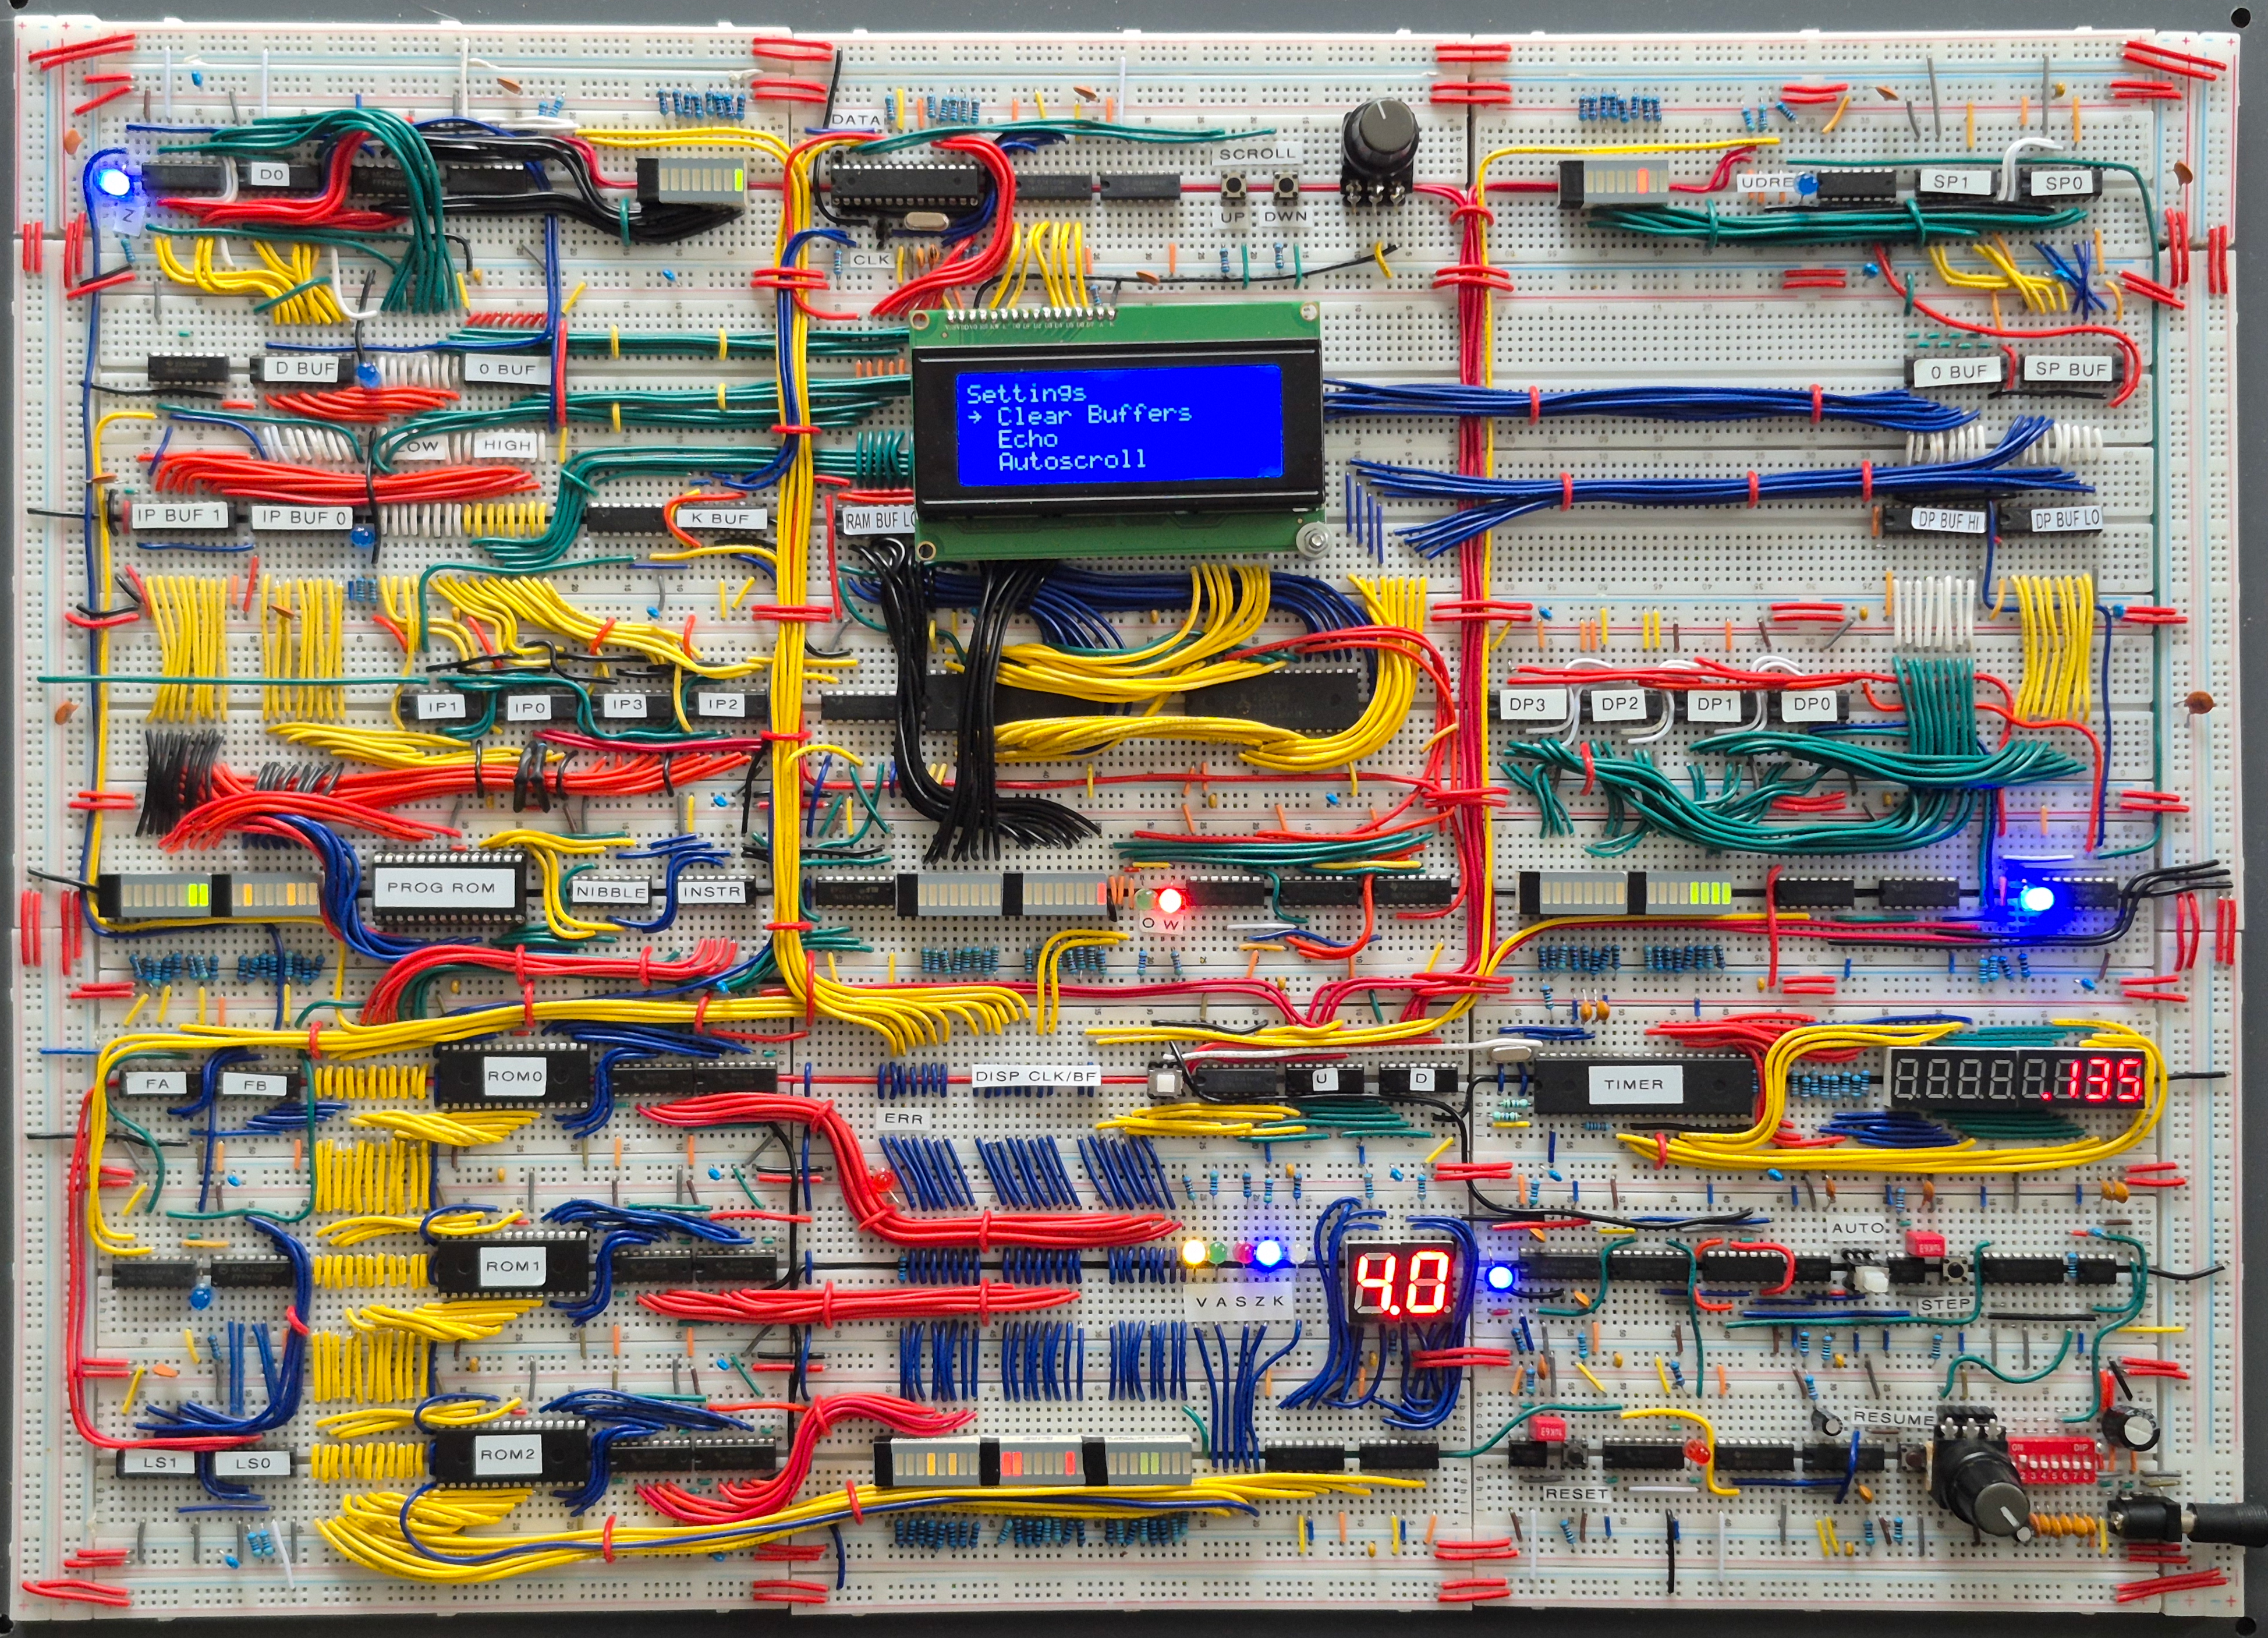
\includegraphics[width=0.8\linewidth]{img/full_board}
    \caption{Prototype of February 2025}
    \label{fig:prototypea}
  \end{subfigure}
  \vspace{\baselineskip}
  \begin{subfigure}{0.9\linewidth}
    \centering
    \includegraphics[width=0.8\linewidth]{img/computerparts}
    \caption{Location of the modules on the prototype}
    \label{fig:prototypeb}
  \end{subfigure}
  \caption{}
  \label{fig:prototype}
\end{figure}

%%%%%%% CLOCK

\subsection{Clock} \label{sec:clock}
\begin{figure}[H]
  \centering
  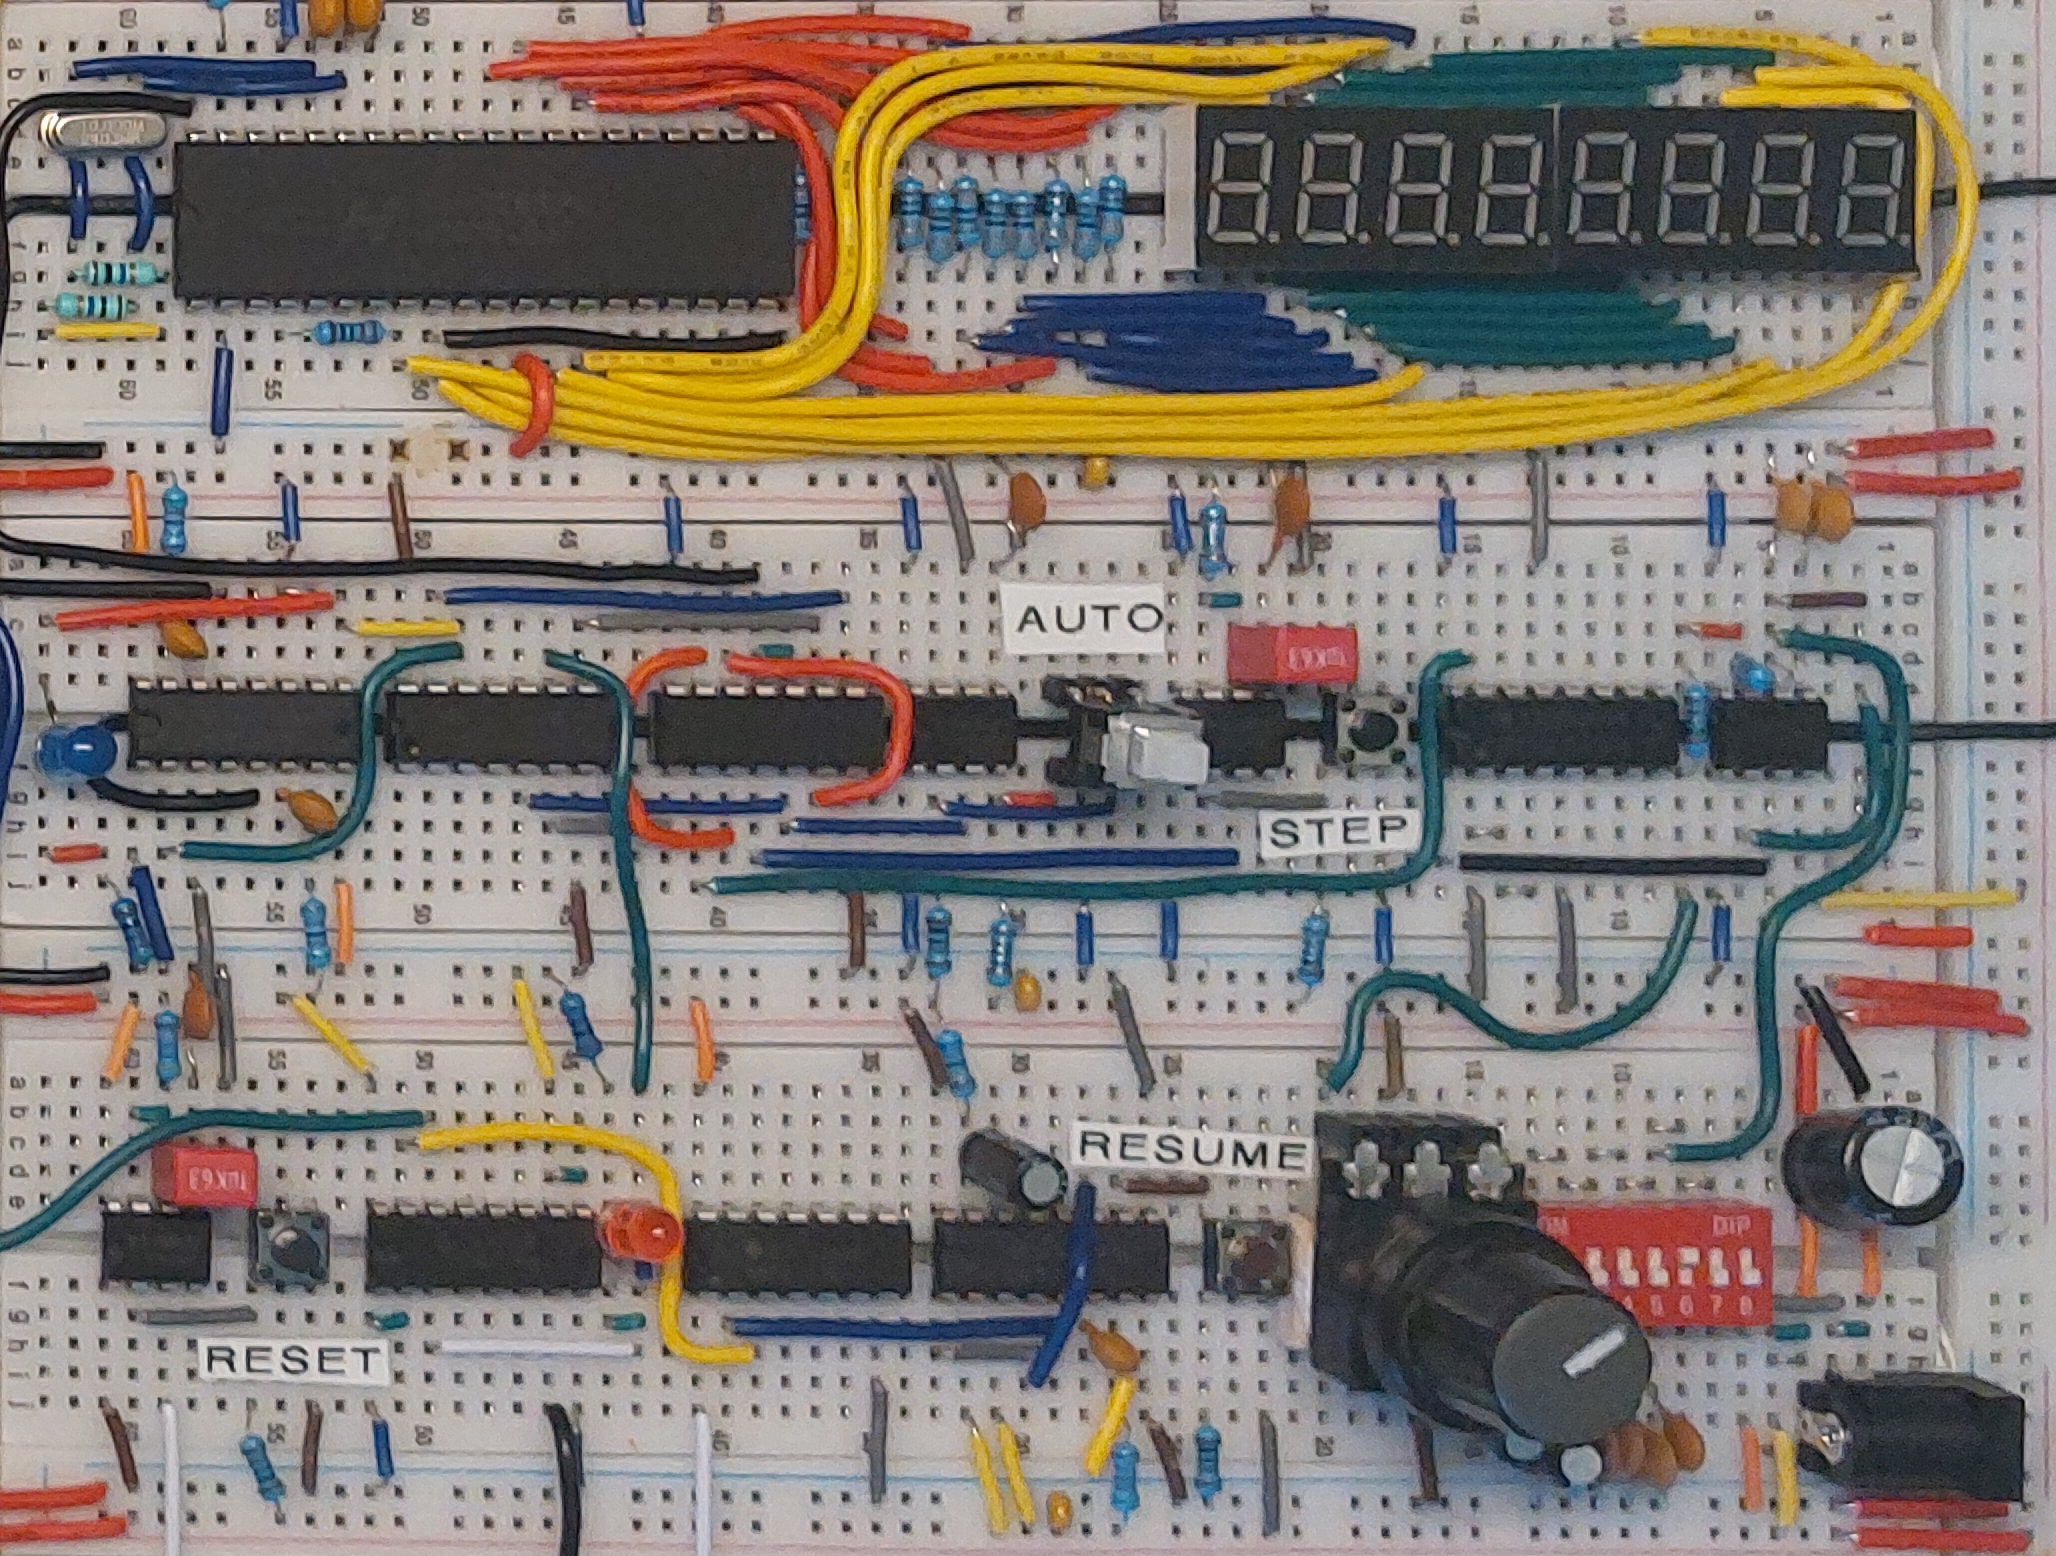
\includegraphics[width=0.6\textwidth]{img/clockmodulecloseup}
  \caption{Close up of the Master Clock and Reset/Resume Modules.}
  \label{fig:masterclockcloseup}
\end{figure}

\subsubsection{Overview}
The clock module is located at the bottom right of the computer and is responsible for providing a heartbeat to (most of) the modules. The core design of the clock, based around a 555 timer in astable mode, is taken directly from Ben Eater's 8-bit computer video's \cite{beneater}. The output frequency can be set using an array of DIP-switches to select the capacitor of an RC-circuit for coarse control and a 10K linear potentiometer for fine control. Two additional 555 timers are used to debounce both the pushbutton for the manual clock and the latching push button which acts as a select between the two modes, as per Ben's design. 

The frequency of the astable 555 is halved by sending it through a JK flip-flop to ensure a perfectly symmetric duty cycle, then fed into a 74LS123 monostable multivibrator to produce two short 200ns pulses: one on the rising and another on the falling edge the output of the flip-flop. This results in two sets of clean signals at constant intervals. On the first pulse (rising edge of the output of the flip-flop), control signals are loaded from the microcode EEPROMs into a set of registers (74LS173) that buffer these control signals for stability; even when the inputs to the EEPROM address-pins change during execution of an opcode, this will not affect the control signals presented at the modules. The second pulse (generated by the falling edge of the flip-flop) is used as a clock to the modules; this is when the modules execute their command, like loading a value into RAM or incrementing the contents of a register. This approach guarantees a clean division between setting the control signals and clocking the modules. Figure \ref{fig:clocktiming} shows the timing diagram for the different signals discussed above.

\begin{figure}[H]
  \centering
  \includegraphics[width=0.6\textwidth]{img/clocktiming}
  \caption{Timing diagram for the clock signals.}
  \label{fig:clocktiming}
\end{figure}

\paragraph{Frequency Control.} The frequency of the master clock can be set using DIP switches to select the capacitor-value and a 10K potentiometer to select the resistance of the RC circuit connected to the 555 timer. The capacitor, in conjunction with a fixed 2K resistor, sets a broad range (lower capacitance corresponding to higher frequencies) while the potentiometer is used fine-grained selection of the frequency within this range. This potentiometer is wired in series with a 1K resistor to ensure stability when the potentiometer resistance drops toward zero. Table \ref{tab:frequencycontrol} shows the frequency-ranges available for each of the currently selected capacitors. These values have been measured \emph{after} the flip-flop (so the actual frequency of the 555 timer is around double the frequencies displayed in table \ref{tab:frequencycontrol}). Having a broad range of frequencies available makes it possible to run at very low speeds for educational purposes, or at very high speeds for complicated, long running algorithms.

\begin{table}
  \centering
  \begin{tabular}{c|r|r}
    Capacitance (F) & $f_{min}$ (Hz) & $f_{max}$ (Hz) \\ \hline
    $10^{-5}$  & 5 & 15 \\
    $10^{-6}$  & 40 & 140 \\
    $10^{-7}$  & 500 & 1,500 \\
    $10^{-8}$  & 5,000 & 14,000 \\
    $10^{-9}$  & 19,000 & 55,000 \\
    $10^{-10}$ & 38,000 & 108,000 \\
    $10^{-11}$ & 90,000 & 270,000 \\
  \end{tabular}
  \caption{Frequency ranges for each of the capacitors (approximate).}
  \label{tab:frequencycontrol}
\end{table}

\paragraph{Frequency Display:} To be able to see the clockfrequency as well as the instruction-frequency (number of BF instructions executed per second), the module clock (M\_CLK) and INC(IP) signals are connected through a switch to the input of an ICM7226B timer chip\cite{?}, which is configured as an 8-digit frequency timer. It drives two 4-digit 7-segment displays at a 1 second interval (the frequency is measured and updated every second). 

\subsection{Reset/Resume} \label{sec:resetresume}
\paragraph{Reset.} The Reset/Resume module is located directly underneath the clock and contains logic necessary to reset the computer (necessary after applying power) or resume the clock after it has been halted. The HLT signal coming from the decoder is latched into a register (74LS173) from which the corresponding output bit is connected to the HLT input of the clock module. When the system is reset (using the reset button) or when the resume button is pressed, the HLT bit is cleared and the clock output is enabled again. This allows for pausing and resuming the computer, effectively adding breakpoints to the code. The reset button itself is debounced in the same way as the manual clock button to ensure a stable transition with a debounce time of around 300ms.

\paragraph{Resume.} The Resume button needs more sophisticated debounce circuitry due to the following scenario: when multiple HLT instructions are seperated by a relatively small amount of other instructions, a pulse in the order of milliseconds (like the reset and pulse debouncers) will be far too long at high clock frequencies. The resume-signal will still be high when a second (or third, fourth, ...) HLT instruction is encountered, causing control flow to simply skip over these instructions. To remedy this situation, a debouncing circuit is required that first produces a pulse of equal width of the clock pulses (Figure \ref{fig:clocktiming}), followed by a guaranteed period where the signal is low, even when the button bounces after the pulse. This is achieved by creating a feedback loop between the two monostable vibrators present on the 74LS123. The first one will produce a 200ns pulse on the rising edge of the button. This pulse is sent to the reset of the register that holds the HLT signal in order to clear it, but is also connected to the second monostable vibrator. When the initial (short) pulse goes low, the second vibrator generates a much longer pulse that is connected to the reset-input of the first one, making sure it cannot be re-activated for some time. By selecting a 680K resistor and a 4.7$\mu F$ capacitor, a cooldown period of around 1 second is achieved. Figure \ref{fig:resumedebounce} shows a timing diagram to illustrate this process in more detail. 

\begin{figure}[H]
  \centering
  \includegraphics[width=0.6\textwidth]{img/resumedebounce}
  \caption{Timing diagram for the resume debouncer. The output of Monostable 1 is connected to the reset of the register that stores the HLT signal.}
  \label{fig:resumedebounce}
\end{figure}


\subsubsection{Schematic}
Full schematics for the clock module, reset/resume circuitry and the frequency display section are provided on the next pages.
\includepdf[landscape=true]{schematics/masterclock.pdf}
\includepdf[landscape=true]{schematics/frequencydisplay.pdf}

%%%%%%% REGISTER DRIVER

\subsection{Register Driver} \label{sec:implementation:registerdriver}
\begin{figure}[H]
  \centering
  \includegraphics[width=0.6\textwidth]{img/registerdrivercloseup}
  \caption{Close up of the Register Driver Module.}
  \label{fig:registerdrivercloseup}
\end{figure}

\subsubsection{Overview}
The register driver is responsible for driving the U- and D-inputs of the 74LS193 counting registers that are used to implement the D, DP, SP, IP and LS register modules. To increment the '193, its D-input needs to be held high whileproviding a low pulse to the U-input. As explained in section \ref{sec:architecture:cu}, a centralized driver was used to limit the number of logic IC's necessary to drive the registers and the total number of control signals necessary.

The driver module uses a pair of 74LS138 decoders: one to drive the U-inputs and the other to drive the D-inputs of the '193. The '138 takes 3 address bits (A, B, and C) to select one of 8 outputs (Y0-Y7), which will be pulled low when selected (all other outputs remain high). Two gate-inputs G1 (active high) G2 (active low) are used to enable the outputs of the chip; the selected output is activated (pulled low) only when both gates are active. This is very convenient given the fact that the 74LS193 needs a low pulse to increment or decrement its value:
\begin{itemize}
\item The register-selects signals RS0, RS1 and RS2 are connected to A, B, and C to select the required output.
\item The INC and DEC signals are connected through inverters to the G2 gate.
\item The module-clock signal is connected to G1: when pulsed, the selected output will produce a pulse that is effectively an inverted clock pulse (high-low-high) which is exactly what the '193 expects. 
\end{itemize}

\subsubsection{Schematic}
A full schematic is provided on the next page.
\includepdf[landscape=true]{schematics/registerdriver.pdf}

%%%%%%% DATA POINTER REGISTER

\subsection{DP Register} \label{sec:implementation:dp}
\begin{figure}[H]
  \centering
  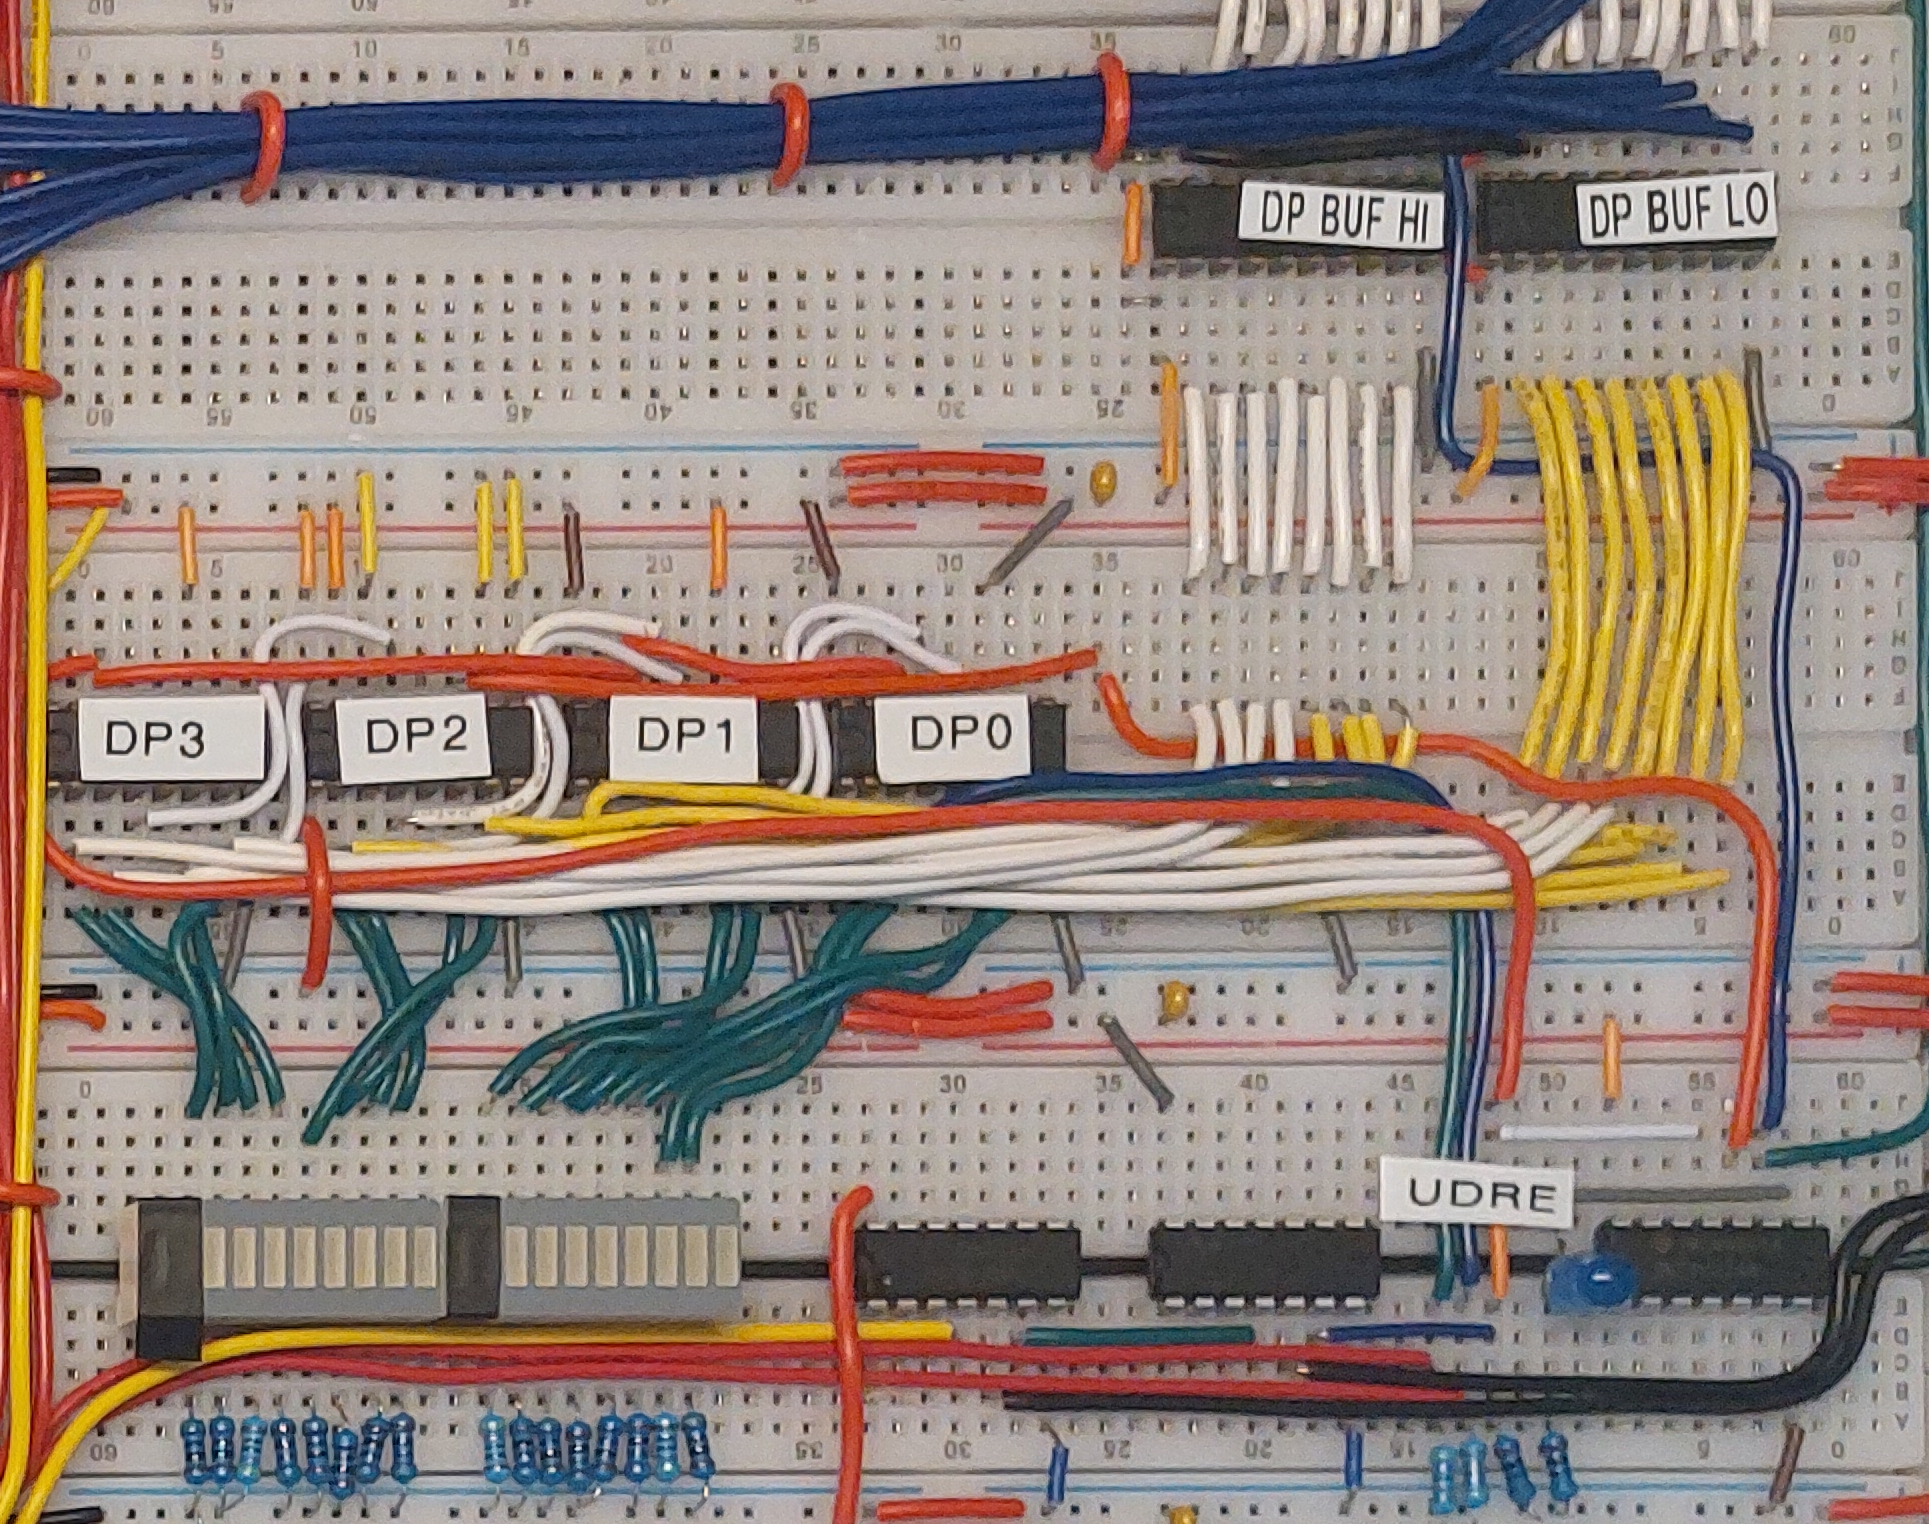
\includegraphics[width=0.6\textwidth]{img/dpregistercloseup}
  \caption{Close up of the Data Pointer Register Module.}
  \label{fig:dpregcloseup}
\end{figure}

\subsubsection{Overview}
The DP Register Module is the module that is responsible for managing the data-pointer; it contains a 16-bit value that is connected to the address bus of the RAM and points to the memorycell currently pointed to by the BF-pointer. The value is stored across four 74LS193 binary counters that are chained together (each holding 4 bits), making it possible to address a total of $2^{16}=65,536$ different memory cells. The DP is connected to the register driver at address 2 (0b010, see Table \ref{tab:registers}) and as such can be incremented or decremented when the program hits a \texttt{>} or \texttt{<} respectively. The outputs of each '193 are connected to the address bus through a pair of tristate buffers (74LS245) to prevent bus contention with the stack pointer; see below (Enabling Ouput) for more information on the enable-signal.

\paragraph{Reset Vector.} Since the data section in RAM starts at 0x0100 (0x0000 through 0x00ff are reserved for the stack), this is the value that the register should start at right after booting up the system (all other registers start out with an initial value of zero). To achieve this, the global reset line of the system is connected to the reset pin of the 193's corresponding to nibbles 0, 1 and 3, but to the load-pin of nibble 2, who's inputs have been hardcoded to 0b0001 (0x1). This register is also special in the sense that it is the only register that needs to reset at runtime (through the CLR\_DP signal), without resetting any of the other modules. After all, after initializing its memory to 0 by looping through (part of) its addressable space, the DP needs to be brought home to the start of the datasection before the main program starts (see also Sections \ref{sec:sequences:init} and \ref{sec:sequences:home}). The global RESET signal is therefor OR'd with the CLR\_DP signal before going to the reset (and load) pins of the IC's.

\paragraph{Enabling Output.} Perhaps somewhat confusingly, the schematic (see below) shows that the SP\_EN signal is used to enable the buffers. Because the DP shares the address-bus with only the stack pointer (SP) -and their outputs should be mututally exclusive- the same signal can be used to enable and disable their respective buffers: when the stack pointer is enabled, the data pointer should be disabled and vice versa. Given that the output-enable-pin of the 74LS245 is active low, the SP\_EN signal can be fed directly into the enable-pin of the DP buffers. On the side of the SP, the same signal goes through an inverter before going into the enable-pin of its respective buffer. By default, when the SP is not enabled, the DP will provide its address to RAM. The address-bus will therefore never be left floating, which has the nice side-effect of always being able to visually see the current value in RAM by the LED's connected to its outputs. 

\subsubsection{Schematic}
A full schematic is provided on the next page.
\includepdf[landscape=true]{schematics/datapointerregister.pdf}

%%%%%%% DATA REGISTER

\subsection{D Register}
\begin{figure}[H]
  % TODO: add annotations to the image
  \centering
  \includegraphics[width=0.6\textwidth]{img/dregistercloseup}
  \caption{Close up of the Data Register Module.}
  \label{fig:dregcloseup}
\end{figure}

\subsubsection{Overview}
The data register (D) holds (a copy of) the value in memory currently pointed to by the datapointer (DP). In the computer, it is located in the top left corner. Like the DP, it is implemented using 74LS193 counting registers and driven by the register driver described in Section \ref{sec:implementation:registerdriver} at address 1 (0b001, see Table \ref{tab:registers}). Since the data is only 8-bits in size, no more than two '193 chips have to be chained together to create the 8-bit register. 

\paragraph{Enabling Output. } The outputs of the '193s are buffered by a single 8-bit tristate buffer (74LS245) before being connected to the databus. Because the databus is 16-bit wide (necessary to store IP-values on the stack), the high-byte is set explicitly to 0 when D is enabled by a second buffer that always outputs zero's. Storing nonzero values in the high-byte of the datasection would not have any consequences for the computation, but would be visually confusing. The buffers are set to output-mode only (even though the register is able to read from the bus as well) because the 193 chips have seperate pins for incoming and outgoing data. The incoming data is read from the bus directly without needing to go through a buffer.

\paragraph{Z-Flag.} This module also produces the Z flag, indicating that it is currently containing the value 0. This is achieved by connecting its outputs through an 8-input NOR gate (MC14078B). The output of this gate is then connected to the FB flag register where it can be latched in by the CU in order to determine the next course of action.

\paragraph{Loading Data.} Because the '193 loads asynchronously, the clock has to be gated with the LD\_D signal through a NAND gate in order to load synchronously with the clock when the LD\_D signal is high (the load-pin on the '193 is active low). The necessity of a NAND gate meant it was easier to also implement any inverters needed in the circuit in terms of NAND gates.


\subsubsection{Schematic}
A full schematic is provided on the next page.
\includepdf[landscape=true]{schematics/dataregister.pdf}

%%%%%%% INSTRUCTION POINTER REGISTER

\subsection{IP Register}
\begin{figure}[H]
  \centering
  \includegraphics[width=0.6\textwidth]{img/ipregistercloseup}
  \caption{Close up of the Instruction Register Module.}
  \label{fig:iregcloseup}
\end{figure}

\subsubsection{Overview}
The instruction pointer register holds a 16-bit value representing the address of an instruction in the program-ROM (implemented using an EEPROM chip (AT28C64B)). The size of the available address space in program-memory is $2^{14}$ instructions, so the two uppermost bits (bits 14 and 15) of the IP are left unused.

\paragraph{Forbidden Decrement.} The IP, like the D and DP registers, is driven by the Register Driver at address 4 (0b100), but should in principle never be decremented; it either moves to the right (next instruction) or jumps back by loading a value from the databus. Its inability to move left (decremented) is not enforced by the hardware itself, but should be taken care of by the microcode implementation.

\paragraph{Reading and Writing Data.} The IP is connected to the databus through two tristate buffers (74LS245) to avoid bus contention with the DP and IO-module. It is connected to this bus in order to write its value to the stack when a loop is entered. When exiting from a loop, a value is read back into the register through a direct connection to this bus (without going through a buffer). Because loading is done asynchronously on the '193, the load signal is NAND'ed with the clock to make loading synchronous again.

\subsubsection{Schematic}
A full schematic is provided on the next page.
\includepdf[landscape=true]{schematics/instructionpointerregister.pdf}

%%%%%%% STACK POINTER REGISTER

\subsection{SP Register}
\begin{figure}[H]
  \centering
  \includegraphics[width=0.6\textwidth]{img/spregistercloseup}
  \caption{Close up of the Stack Pointer Register Module.}
  \label{fig:spregcloseup}
\end{figure}

\subsubsection{Overview}
The stack pointer (SP) holds an 8-bit value in the range 0x00 - 0xff, which corresponds to addresses within the stack-space of RAM, where IP values can be stored and loaded from when the system sees the \texttt{[} and \texttt{]} loop-instructions. When a loop is entered, the IP register stores its value on the stack at the address pointed to by the SP. The SP then increments its value, ready for the next value to be stored on the stack when a nested loop is encountered. It is therefore implemented using the 74LS193 binary counter and connected to the register driver at address 3 (0b011). The SP module is connected to the same RAM address bus as the DP, which means it should go through a tristate buffer to avoid bus contention. As mentioned before (\ref{sec:implementation:dp}), the SP buffer shares its enable-line (though inverted) with the DP. A second buffer that, when enabled, only outputs zero's on the address-bus is used to make sure that only the stack is addressed by the SP and no accidental reads or write happen in the datasection. 


\subsubsection{Schematic}
A full schematic is provided on the next page.
\includepdf[landscape=true]{schematics/stackpointerregister.pdf}


%%%%%%% LS Register

\subsection{LS Register}
\begin{figure}[H]
  \centering
  \includegraphics[width=0.3\textwidth]{img/lsregistercloseup}
  \caption{Close up of the Loop Skip Register Module.}
  \label{fig:spregcloseup}
\end{figure}

\subsubsection{Overview}
The Loop Skip Register (LS) is used to produce the loop-skip-flag (S, see \ref{sec:architecture:ls}). It is implemented using two 74LS193 binary counters and is connected to register driver at address 5 (0b101). Like the Z-flag, the S-flag is produced by sending the outputs of the binary counters through an 8-input NOR-gate, the output of which is then inverted and connected to the FB flag-register. When any of these bits are high, the S flag will be raised, indicating that the computer is in the process of skipping the current loop.


\subsubsection{Schematic}
A full schematic is provided on the next page.
\includepdf[landscape=true]{schematics/loopskipregister.pdf}


%%%%%%%%%%% FA/FB

\subsection{Flag Registers}
\begin{figure}[H]
  \centering
  \includegraphics[width=0.6\textwidth]{img/flagregistercloseup}
  \caption{Close up of the flag registers FA and FB.}
  \label{fig:ramcloseup}
\end{figure}

\subsubsection{Overview}
There are two stages of flag-buffering; the first stage is the FA register (in which the A and V flags are stored) and the second the FB register (in which all flags except K are latched when the instruction is loaded). Both of these registers have been implemented using a 74LS173 4-bit register. The A and V flag are stored in FA by the CU whenever the value in D is changed (V) or whenever the pointer is changing its position (A). This can happen mid-instruction without changing the address on the microcode EEPROMs because the flag lines leading into those come from the FB register. At each cycle 0, the buffered A and V flags are loaded into FB, together with S and Z coming from the LS and D registers respectively. Since this always happens in conjunction with loading the instruction from program ROM into the instruction register (see \ref{sec:implementation:cu}), the control signal has been named LD\_FBI. The flags in the FB register will (mostly) remain constant during the execution of an opcode.

\subsubsection{Schematic}
A full schematic is provided on the next page.
\includepdf[landscape=true]{schematics/loopskipregister.pdf}


%%%%%%% RAM Module

\subsection{RAM}
\begin{figure}[H]
  \centering
  \includegraphics[width=0.6\textwidth]{img/ramcloseup}
  \caption{Close up of the RAM Module.}
  \label{fig:ramcloseup}
\end{figure}

\paragraph{Capacity} The RAM module is mainly used to store the 8-bit data of the BF memory-tape. However its secondary purpose is to also store the instruction-pointer values when loops are handled, which are 16-bit in size. Therefore the RAM module contains two 512K x 8-bit SRAM chips (AS6C4008) for a total of 512K 16-bit memory-cells. The second chip is therefor only used to store the high-byte of the IP's stored on the stack (at most 256 values). The remainder of the capacity of this chip is not used at all, since the datavalues are only 8 bits in size.

\paragraph{Buffering} The AS6C4008 already provides a Chip Enable input which is supposed to be used when the data is connected to a databus. When this input is inactive, its outputs are in a high impedance state to avoid bus contention with other devices. However, in this project we need the data currently pointed to to be visible on an array of LED's, which means that the chip should be enabled basically at all times (except when writing to it). Additional logic is used in conjunction with a pair of 74LS245 tristate buffers to intercept the outputs before making them available on the bus through the buffers. The truthtable for this logic is incorporated in the schematics below. The LED's are not shown in the schematic, but can be connected directly to the datalines of the RAM in this configuration. 

\subsubsection{Schematic}
A full schematic is provided on the next page.
\includepdf[landscape=true]{schematics/rammodule.pdf}


%%%%%%% CONTROL UNIT

\subsection{Control Unit}\label{sec:implementation:cu}
\begin{figure}[H]
  \centering
  \includegraphics[width=0.6\textwidth]{img/controlunitcloseup}
  \caption{Close up of the Control Unit.}
  \label{fig:controlunitcloseup}
\end{figure}

\subsubsection{Overview}
The control unit is responsible for sending the appropriate control-signals to each of the modules. The general idea is that the current instruction pointed to by the IP (4 bits) together with the state flags (another 5 bits: K, A, V, S and Z) and the cycle count (3 bits) combine together to form a 12-bit address into a set of three EEPROM chips (AT28C64B), each of which contains part the signal configuration corresponding to the current state of the system. When clocked by the decoder-clock (D\_CLK), the values currently at this address are loaded into six 74LS173 registers (two per EEPROM) and asserted onto their respective modules, which will act upon them on the next pulse of the M\_CLK signal.

\paragraph{Address Layout.} Based on the physical layout of the board, the following configuration was used to construct an address into the EEPROMs.
\\
\begin{center}
\begin{tabular}{r|ll} 
  Address Bits & \\ \hline
  0-2  & Cycle count & ($000_2$ - $111_2$) \\
  3-7  & Instruction & ($0000_2$ - $1111_2$) \\
  8-12 & Flags  & ($00000_2$ - $11111_2$) \\
  13   & Unused & 
\end{tabular}
\end{center}


\paragraph{Generating and Programming Microcode.} The three EEPROM's have been programmed using a custom built EEPROM programmer based around an Arduino Nano, combined with a python script (\texttt{bflash.py}) that is able to send a binary image to the Nano over a serial connection. The images that store the microcode tables have been generated by Mugen (see \ref{sec:utilities:mugen}), a utility developed to make the microcode programming more maintainable. Mugen generates the images from a specification file. The relevant part of the specification for the Synapse-191 is shown in the listing below and is a direct representation of the microcode shown in Table \ref{tab:microcode}.

\newpage
\lstinputlisting[style=MugenStyle, firstline=58, firstnumber=1]{../src/microcode/bfcpu.mu}


\paragraph{Instruction Nibbles.} The actual BF program is stored in another 8K EEPROM chip (AT28C64) and is addressed by the instruction pointer as mentioned before. Since each BF instruction only needs 4 bits to be encoded (there are less than 16 different opcodes), we can store up to 16K instruction in the chip by packing 2 consecutive instructions together in a single byte (handled by the assembler, \texttt{bfasm}). Rather than using bit 0 from the IP directly as address bit 0 on the EEPROM, it is used as the data-select signal to a 74LS157 multiplexer. This multiplexer takes 1 select-bit and two sets of 4 databits. Depending on the value of the select-bit, one of the sets of 4-bit data is sent to its outputs. This allows us to select either the low or high nibble of the data in the EEPROM, effectively doubling the amount of instructions that can be stored and retrieved.

\paragraph{Instruction Register.} The seleted nibble is loaded into the instruction register (I) at the same time as the V, A, S and Z flags are loaded into the FB register. For this reason both the FB and I registers can operate on the same control-signal: LD\_FBI. The I register is implemented using the 74LS161, which is actually a counting register, because at the time there was no '173 available anymore and these chips are functionally almost identical when counting is disabled on the '161. Initially, the outputs of the multiplexer ('157) were directly connected to the address lines of the microcode EEPROMs but when it turned out that this could cause instabilities in some rare occasions, the I register was added to buffer the instruction for the entire duration of the opcode execution.
 
\paragraph{Cycle Counter.} The cycle counter is implemented by a 74LS161 binary counter that simply increments on every M\_CLK signal up and sends its outputs (bits 0-2) to address lines 0-2 of the microcode EEPROM chips. It is reset when it receives the CR signal (which becomes active when after an instruction has completed).


\subsubsection{Schematic}
A full schematic is provided on the next page.
\includepdf[landscape=true]{schematics/controlunit.pdf}

%%%%%%% IO Module
\subsection{IO Module} \label{sec:implementation:io}
\begin{figure}[H]
  \centering
  \includegraphics[width=0.6\textwidth]{img/iomodulecloseup}
  \caption{Close up of the IO Module.}
  \label{fig:iomodulecloseup}
\end{figure}

\subsubsection{Overview}
The IO system is handled by an ATMEGA328P microprocessor, commonly found in the Arduino Uno. It has four main functions:
\begin{enumerate}
\item Drive the screen and display contents from the bus when instructed to by the \texttt{EN\_OUT} signal.
\item Handle keyboard input and provide input data to the bus when instructed to by the \texttt{EN\_IN} signal.
\item Provide a random number to the bus when both signals are supplied (implementing the \emph{Random Brainf*ck Extension}).
\item Supply a menu system to alter its settings using two buttons.
\end{enumerate}

\paragraph{Buttons and Menu} Two buttons are provided to interact with this system. They are mainly used to scroll the screen but can also be used to access and navigate a menu (Figure \ref{fig:menuscreen}). This menu let's the user do the following:
\begin{enumerate}
\item Clear the screen and keyboard buffer.
\item Change the display-mode. By default, incoming data is interpreted as ASCII characters. When it should be displayed as raw numerical values (either in base 10 or 16), this option can be selected from the menu. When in either of these numerical modes, a delimiter character can be selected to separate bytes visually.
\item Set autoscrolling on/off. By default the screen will scroll its contents when they overflow to always keep the most recent data in view. When new data is displayed, the screen is always scrolled to display this data. Setting autoscroll to `off' will disable these features.
\item Echo on/off. When running an interactive program that requires keyboard input, the user probably wants to see what is being typed. This is the default behavior (echo on). If for some reason the keypresses should not be displayed, this option can be disabled.
\item Set the input-mode. By default, the IO module will wait for the input-buffer to contain a value before putting anything on the bus and notifying the CU throught the K-flag (buffered input-mode). However, an alternative mode (immediate) can be selected, in which case the IO module will put a zero on the bus when the buffer is empty and set the K-flag regardless. This can be helpful if programs require real-time inputs (e.g. for simple games).
\item Set the RNG seed. For programs that use the Random Number Generator as an input device, the seed can be set through this option. Since the same seed will produce the same sequence of numbers, this option can be used to control the randomness of the application. A `true' random seed can normally be emulated by seeding the generator with the reading of a floating analog input for example, but sadly no free analog inputs were left available on the MCU.
\item Reset to default settings. Whenever settings have been changed, the new settings will be saved to the persistent EEPROM memory of the MCU and loaded back on startup to make the settings persist when the MCU is powered down. This option allows you to revert all changes and load the default settings back in.
\end{enumerate}

\begin{figure}[h]
  \centering
  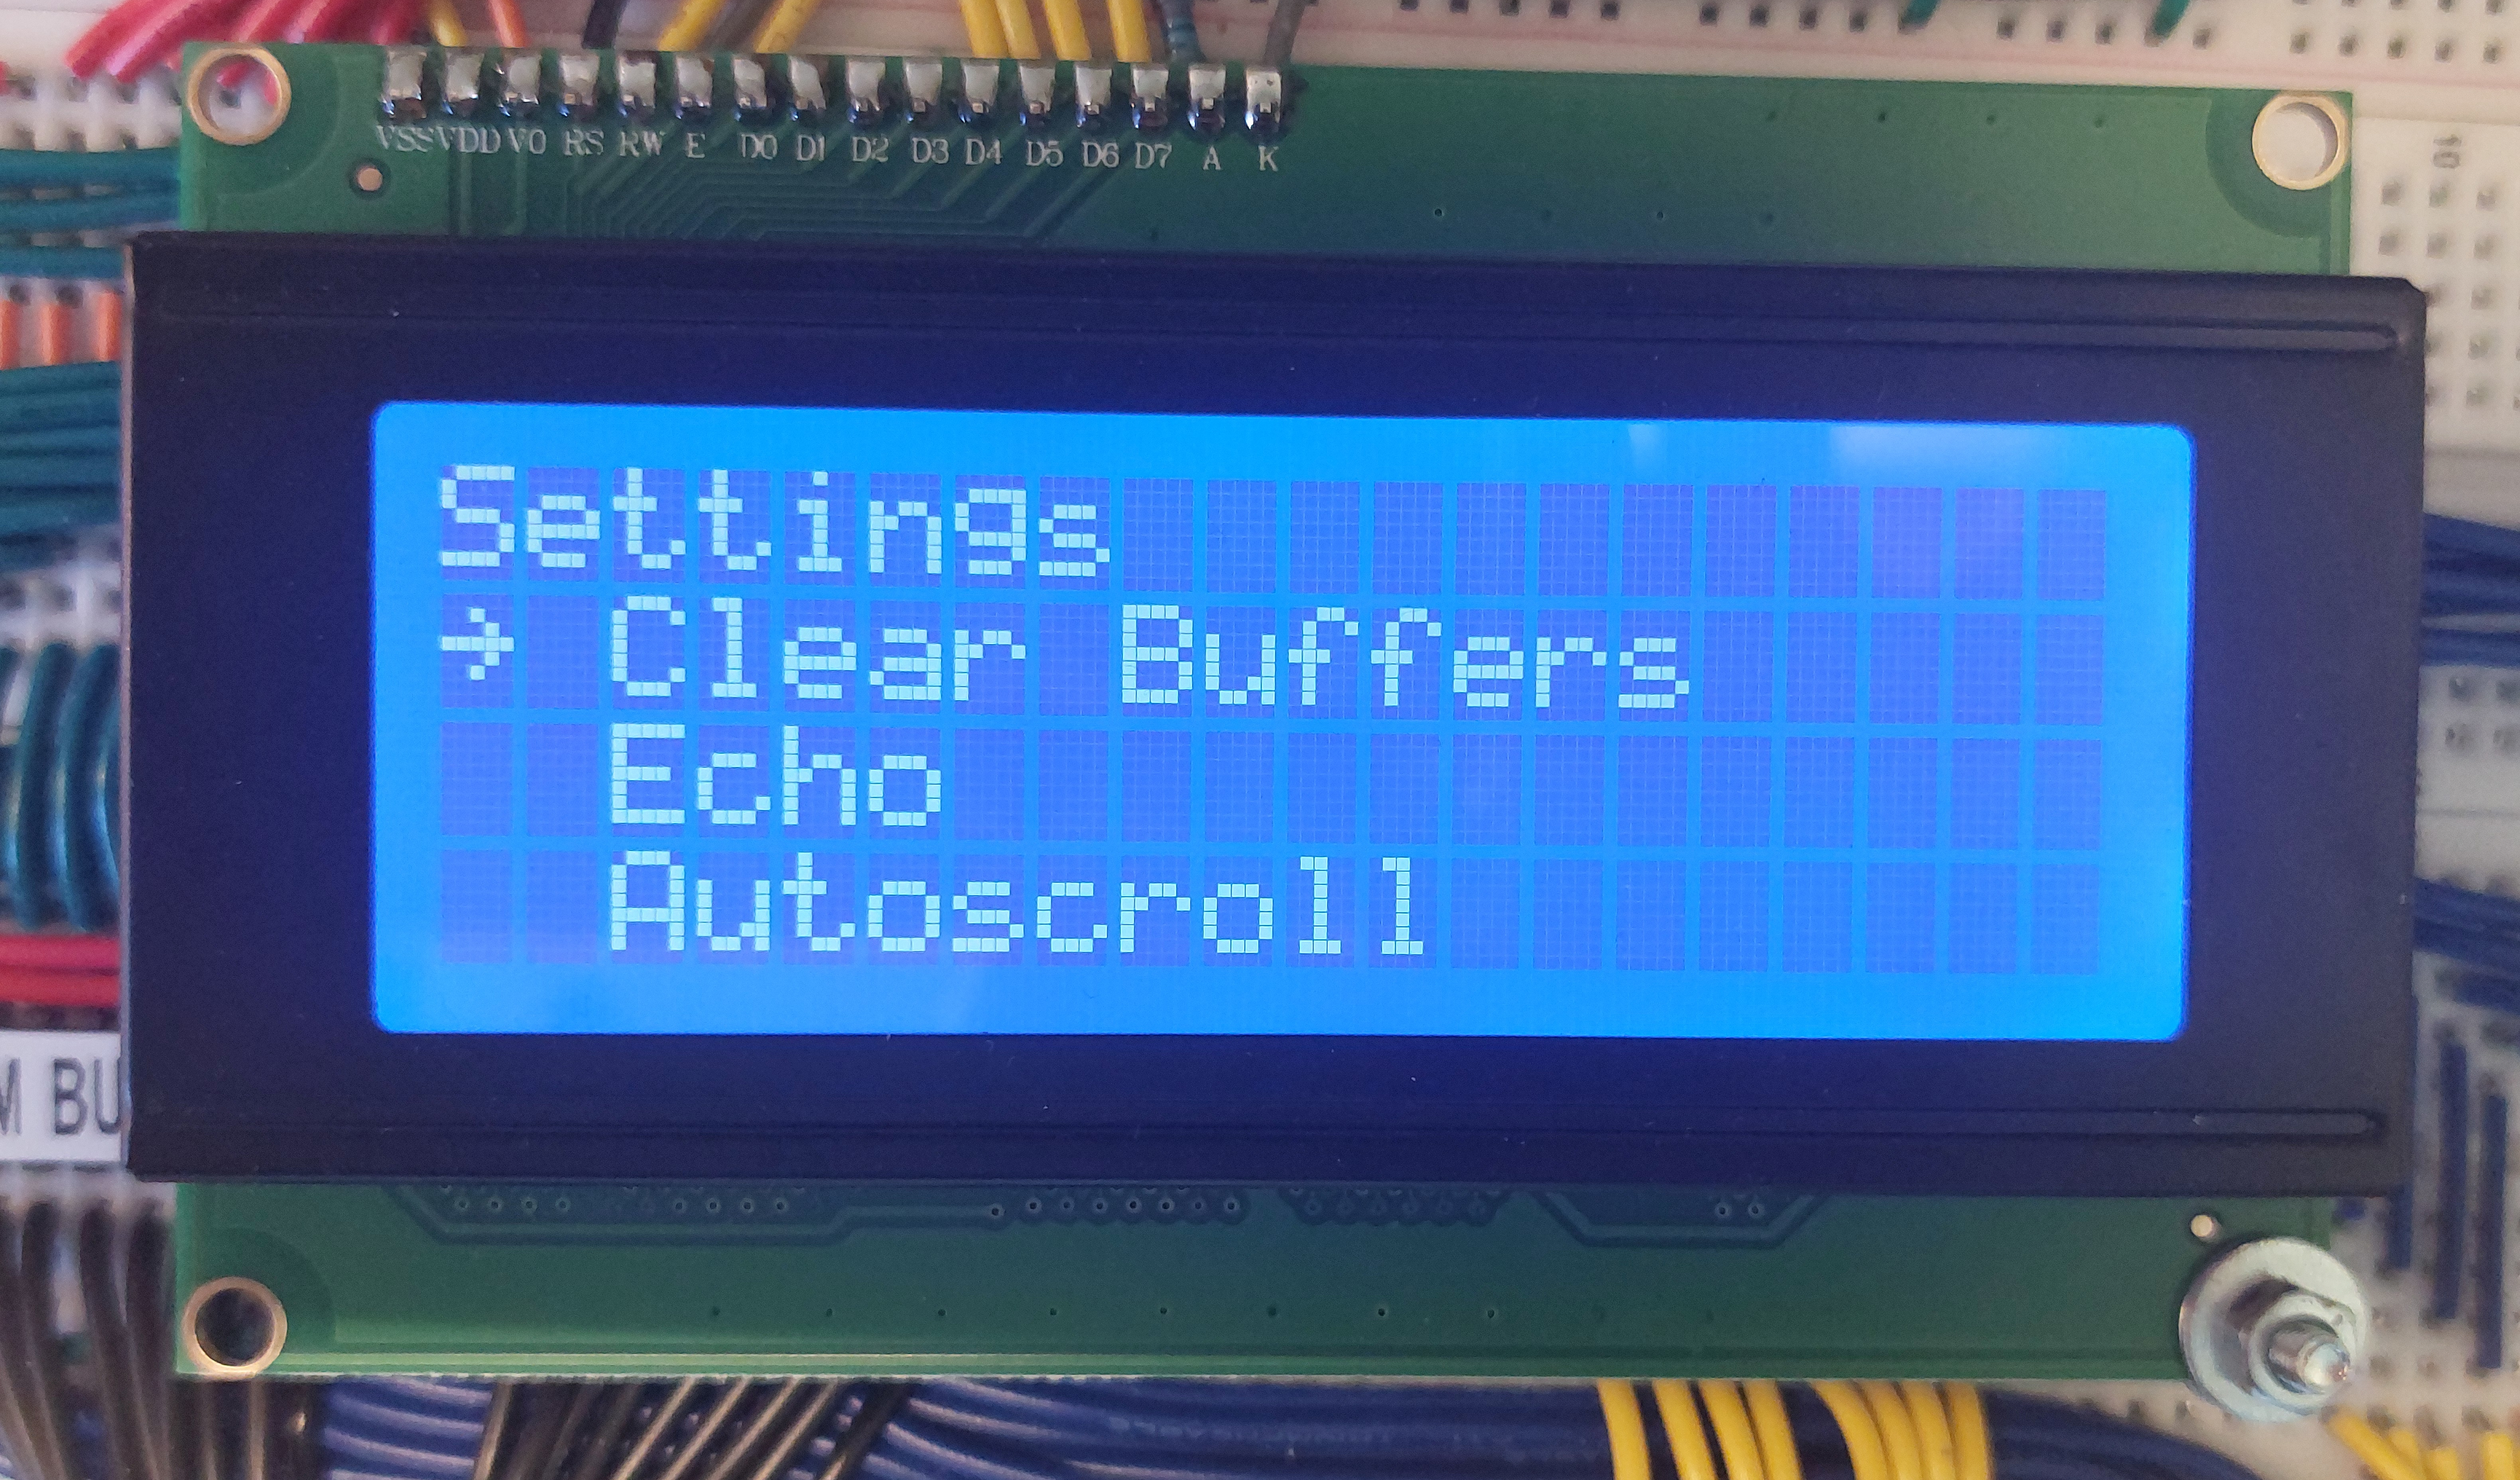
\includegraphics[width=0.5\textwidth]{img/menuscreen}
  \caption{Part of the menu that is accessible by pressing both scroll-buttons simultaneously.}
  \label{fig:menuscreen}
\end{figure}


\subsubsection{Handshake Protocol}
\paragraph{Output} The \texttt{M\_CLK} signal is connected to an interrupt pin of the MCU. On every interrupt triggered by the clock, when the system is in its IDLE state, it will check the EN\_IN and EN\_OUT lines to determine if it should initiate a read or write sequence to the databus. When EN\_OUT is found to be high, it will copy the byte currently present on the bus into its screen-buffer, set the K flag and change its state to WAIT\_SYS. On every subsequent clock pulse, while in the WAIT\_SYS state, it will check if the K flag has been reset by the control unit. If so, the handshake has been completed and the module returns to its IDLE state (see Figure \ref{fig:isrflow}).

\paragraph{Input} If the EN\_IN signal is found to be asserted, the system has two possible courses of action, depending on the input-mode currently set by the user (through the on-screen settings menu). In (the default) buffered mode, the system will change its state to WAIT\_KB and wait for a byte to become available in the keyboard-buffer. As soon as it does, it will provide this value onto the bus and notify the CU by setting the K flag. It then moves into the WAIT\_SYS state to await confirmation by the CU (which in turn resets the K flag). In immediate mode, all zeros will be written to the bus and the K flag is set immediately even when the keyboard-buffer is still empty. If, in addition to EN\_IN, EN\_OUT is asserted as well, a random byte is put onto the bus (see Figure \ref{fig:isrflow}).

\begin{figure}[H]
  \centering
  \includegraphics[width=\textwidth]{img/isrflow}
  \caption{Control flow inside the ISR running on the microcontroller.}
  \label{fig:isrflow}
\end{figure}

\subsubsection{Shift Register}
A shift register (74HC595) had to be used to decrease the number of pins on the Atmega328p necessary to drive the LCD screen. Not a single IO pin has not been used, so the shift register proved invaluable for this application.

\subsubsection{LCD Screen}
The software was written in such a way that most common LCD character screens (compatible with Hitachi the HD44780 driver) will be handled appropriately. Both a 16x2 and 20x4 have successfully been installed in the computer. A modified version of the \texttt{LiquidCrystal\_74HC595} library was used to implement the LCD driver.

\subsubsection{Keyboard}
The IO module can only handle input from PS/2 compatible keyboards. A modified version of the \texttt{PS2Keyboard} library was used to implement the keyboard driver.

\subsubsection{Software}
The full source code for the IO module can be found on Github: \url{https://github.com/jorenheit/bfcpu/tree/main/src/io_module}.

\subsubsection{Schematic}
A full schematic is provided on the next page.
\includepdf[landscape=true]{schematics/iomodule.pdf}

\section{Algorithms}\label{section:algorithms}
The BFX compiler implements a series of algorithms to perform basic operations on the data stored in the data-array, which map to common operators and statements in most programming languages. This section will document each of these algorithms, starting with the most fundamental ones, which we can then use to implement the more complex operations. In the process, we will develop a pseudo language that maps directly to BF-code. The statements of the pseudo language will always be written within a set of curly braces, in order to seperate them from the BF operators.

\tocless\subsection{Moving the Pointer: \texttt{\{x\}}}
Whenever we need to operate on a cell, we first need to move the datapointer to this cell. It is assumed that the compiler is aware of the current pointer position and will therefore be able to move the pointer to any other cell, as long as the address of this cell is also known at compile-time. From now on, the operation of moving to a cell designated by some variable \texttt{x} will be written in as \texttt{\{x\}}.

\textbf{In future expressions enclosed by curly braces, the pointer is always left implicitly at the address of the left-hand-side operand.}

\tocless\subsection{Setting a Fixed Value: \texttt{\{x <- n\}}}
The next elementary operation is setting some cell to a specific (known) value. We will not assume any prior knowledge of the current contents of this cell, which means the first step is to clear it completely, which we can do by iteratively decrementing the cell until it becomes zero: \texttt{[-]}. We then follow it up by the desired amount of increments. For example, setting cell \texttt{x} to \texttt{5} can be done with:
\begin{lstlisting}
  {x} [-] +++++
\end{lstlisting}
From now on, we will use the following shorthand for setting a cell (\texttt{x}) to a fixed value (n): \texttt{\{x <- n\}}.
\tocless\subsubsection{Using \texttt{+} Instead: \texttt{\{x <- n+\}}}
Instead of decrementing the cell until it becomes zero, we could also choose to increment it using \texttt{[+]}. The cell will eventually overflow and wrap back to zero, achieving the same result. This might seem unnecessary and dangerous, especially for 16-bit or larger values, because it can take a lot of time before the cell overflows. However, for some algorithms, where a cell is intentionally being \emph{underflown}, this is a helpfull tool to have at hand. When we need it, we will use a slightly different shorthand: \texttt{\{x <- n+\}}.

\tocless\subsection{Moving Data: \texttt{\{x <- y\}}}
It turns out that moving data is a lot easier than copying data. When moving data from one cell to another, the source-cell will be left empty. Below is a listing for the algorithm that moves the contents of cell x into cell y, leaving cell x empty after the move:
\begin{lstlisting}
  {y <- 0} 
  {x} [ {y} + {x} - ]
\end{lstlisting}
After clearing \texttt{y}, we move the pointer to \texttt{x} and decrement it until it becomes zero, while at the same time incrementing cell \texttt{y}. This algorithm can be extended to move the data into arbitrarily cells, simply by adding variables to the loop and incrementing those as well. Moving data from \texttt{x} to \texttt{y, z, ...} will from now on be written as \texttt{\{(y, z, ...) <- x\}}, analogous to moving a fixed value into a cell.

\tocless\subsection{Assignment/Copy: \texttt{\{x = y\}}}
An assignment of the form \texttt{x = y} will assign the contents of cell \texttt{y} to cell \texttt{x}, overwriting the previously present value of \texttt{x}. This can be achieved by moving the contents of \texttt{y} into both \texttt{x} and a temporary value \texttt{tmp}. This will leave \texttt{y} empty, but we can restore it by moving the contents of \texttt{tmp} back into \texttt{y}.
\begin{lstlisting}
  {(x, tmp) <- y}
  {y <- tmp}
\end{lstlisting}
The shorthand for this operation will from now on be: \texttt{\{x = y\}}

\tocless\subsection{Addition}
\tocless\subsubsection{In-Place Addition: \texttt{\{x += y\}}}
It turns out that adding some value to a cell looks just like a copy, but without resetting the target cell first. Below is the pseudocode for adding the contents of \texttt{y} to \texttt{x}, leaving \texttt{y} intact.
\begin{lstlisting}
  {tmp <- 0}
  {y} [ {x} + {tmp} + {y} - ]
  {y <- tmp}
\end{lstlisting}
This operation will be denoted as \texttt{\{x += y\}}.

\tocless\subsubsection{Return Variable: \texttt{\{z <- x + y\}}}
Rather than adding the contents of a cell to another one and changing the value of the cell on the receiving end, we should also have an algorithm that stores the sum in a new cell, leaving both operands untouched (or at least unchanged). This can be achieved simply by copying the contents of one of the cells to a third cell and applying the addition algorithm:
\begin{lstlisting}
  {z = x}
  {z += y}
\end{lstlisting}

\tocless\subsubsection{Subtraction}
Subtraction works exactly analogously to addition: we just replace the + with a -. This leads to the following shorthands:
\begin{itemize}
\item \texttt{\{x -= y\}} for subtracting a cell in-place and
\item \texttt{\{z = x - y\}} for storing the difference in a return-variable.
\end{itemize}

\tocless\subsection{Multiplication}
Multiplication can be implemented as repeated addition, for which we already have the tools. The same strategy will be used as before, where we first develop an algorithm aimed at multiplying a cell in-place.
\tocless\subsubsection{In-Place Multiplication: \texttt{x *= y}}
To multiply \texttt{x} by the value stored in \texttt{y}, we need to add \texttt{x} to itself, \texttt{y} times. To achieve this, we copy the value of \texttt{y} to a temporary cell, which we can decrement while adding a copy of the original value of \texttt{x} to itself:
\begin{lstlisting}
  {xCopy = x}
  {yCopy = y}
  {yCopy}
  [
    {x += xCopy}
    {yCopy} -
  ]
\end{lstlisting}

\tocless\subsubsection{Return Variable: \texttt{\{z <- x * y\}}}
Like before, we can copy the value of one of the operands into the return address and apply the in-place multiplication algorithm:
\begin{lstlisting}
  {z = x}
  {z *= y}
\end{lstlisting}

\tocless\subsection{Logical Operators}
\tocless\subsubsection{NOT: \texttt{\{x <- NOT y\}}}
The NOT operator basically checks whether the argument is 0, in which case it returns 1. In all other cases, it should return a zero. This can be implemented using the loop-operators, which are the only conditional instructions available to us in BF.
\begin{lstlisting}
  {x <- 1}
  {yCopy = y}
  [
    {x     <- 0}
    {yCopy <- 0}
  ]
\end{lstlisting}

\tocless\subsubsection{AND: \texttt{\{z <- x AND y\}}}
The AND operator will only return 1 when both arguments (x and y) are nonzero:
\begin{lstlisting}
  {z <- 0}
  {yCopy = y}
  {xCopy = x}
  [
    {yCopy}
    [
      {z     <- 1}
      {yCopy <- 0}
    ]
    {xCopy <- 0}
  ]
\end{lstlisting}

\tocless\subsubsection{OR: \texttt{\{z <- x OR y\}}}
The OR operator returns a 1 when either of its arguments are nonzero:
\begin{lstlisting}
  {z <- 0}
  {xCopy = x}
  [
    {z     <- 1}
    {xCopy <- 0}
  ]
  {yCopy = y}
  [
    {z     <- 1}
    {yCopy <- 0}
  ]
\end{lstlisting}

\tocless\subsubsection{Greater Than: \texttt{\{z <- x > y\}}}
To check whether x has a higher value than y, we simply decrement x until it becomes 0. At each step, we also decrement y and check whether it is being decremented beyond zero (check for underflow). If that happens, this means that x is indeed the biggest.
\begin{lstlisting}
  {z <- 0}
  {underflow <- 0}
  {yCopy = y}
  {xCopy = x}
  [
    {underflow <- NOT yCopy}
    {yCopy} -
    {z <- z OR underflow}
    {underflow}
    [
      {yCopy <- 0+}
      {underflow <- 0}
    ]
    {xCopy} -
  ]
\end{lstlisting}

\tocless\subsubsection{Less Than: \texttt{\{z <- x < y\}}}
The less than algorithm can just be expressed as a greater than algorithm, for which the arguments have been swapped around. It will therefore not be repeated below.

\tocless\subsubsection{Equals: \texttt{\{z <- x == y\}}}
Once the `greater than` and `less than` operators have been properly defined, the `equals` operator can be defined in terms of these:
\begin{lstlisting}
  {z <- {NOT x < y} AND {NOT (x > y)}}
\end{lstlisting}

\tocless\subsection{Division and Modulo: \texttt{\{(div, mod) <- x / y\}}}
Division and modulo are done in a single algorithm. Division is implemented as a series of subtractions, counting how many times the numerator fits in the denominator. Two special cases are handled:
\begin{enumerate}
\item When the numerator is zero, the division algorithm is skipped and zero is returned.
\item When the denominator is zero, the algorithm is skipped and the maximum cell value is returned (which is as close to infinity as we can get).
\end{enumerate}
To indicate whether either of these special cases was handled, we set a flag (the loop-flag) which is reset while handling these cases. Only when this flag is still set will the division algorithm be executed. Below is the pseudocode for the expression \texttt{\{(div, mod) = x / y\}}, where \texttt{div} is the result of the division and \texttt{mod} is the remainder after the division.

\begin{lstlisting}
  {div <- 0}
  {mod <- 0}
  {zeroFlag <- 1}  
  {loopFlag <- 1}

  # Special case 1: denominator is 0
  # ==> return max value (255 on 8-bit arch)
  {zeroFlag <- NOT y}
  [
    {div <- 255}
    {mod <- 255}
    {loopFlag <- 0}
    {zeroFlag <- 0}
  ]

  # Special case 2: the numerator is 0
  # ==> return 0 (even in 0/0 case)
  {zeroFlag <- NOT x}
  [
    {div <- 0}
    {mod <- 0}
    {loopFlag <- 0}
    {zeroFlag <- 0}
  ]

  # Division algorithm: repeated subtraction
  {xCopy = x}
  {yCopy = y}

  {loopFlag}
  [
    {xCopy} -
    {yCopy} -
    {mod}   +

    # yCopy became 0?
    # ==> increase result by one and reset yCopy
    {zeroFlag <- NOT yCopy}
    [
      {div} +
      {mod <- 0}
      {yCopy = y}
      {zeroFlag <- 0}
    ]

    # xCopy became 0?
    # ==> done
    {zeroFlag <- NOT xCopy}
    [
      {loopFlag <- 0}
      {zeroFlag <- 0}
    ]
    {loopFlag}
  ]    
\end{lstlisting}

    

\begin{thebibliography}{99} \label{resources}
\bibitem{bfwiki} WikiPedia, \emph{Brainfuck}, https://en.wikipedia.org/wiki/Brainfuck
\bibitem{esolang} Esolanh, \emph{Brainfuck}, https://esolangs.org/wiki/Brainfuck
\bibitem{vonneumann-wiki} Wikipedia, \emph{Von Neumann Architecture},\\https://en.wikipedia.org/wiki/von\_neumann\_architecture
\bibitem{beneater} Ben Eater, \emph{Build an 8-bit computer from scratch}, https://eater.net/8bit
\bibitem{brainfix} Joren Heit, \emph{Brainfix}, https://github.com/jorenheit/brainfix
\bibitem{data-sheets} All data-sheets are available online in the pdf format.
\end{thebibliography}



%etc for each chapter -> easier to maintain


\end{document}
